%%%%%%%%%%%%%%%%%%%%%%
\documentclass{singlecol-new}
\usepackage[utf8]{inputenc}
\usepackage{grffile}


\usepackage{natbib,stfloats}
\usepackage{mathrsfs}

\def\newblock{\hskip .11em plus .33em minus .07em}

\theoremstyle{TH}{
\newtheorem{lemma}{Lemma}
\newtheorem{theorem}[lemma]{Theorem}
\newtheorem{corrolary}[lemma]{Corrolary}
\newtheorem{conjecture}[lemma]{Conjecture}
\newtheorem{proposition}[lemma]{Proposition}
\newtheorem{claim}[lemma]{Claim}
\newtheorem{stheorem}[lemma]{Wrong Theorem}
\newtheorem{algorithm}{Algorithm}
}

\theoremstyle{THrm}{
\newtheorem{definition}{Definition}[section]
\newtheorem{question}{Question}[section]
\newtheorem{remark}{Remark}
\newtheorem{scheme}{Scheme}
}

\theoremstyle{THhit}{
\newtheorem{case}{Case}[section]
}

\makeatletter
\def\theequation{\arabic{equation}}

%\JOURNALNAME{\TEN{\it Int. J. System Control and Information
%Processing,
%Vol. \theVOL, No. \theISSUE, \thePUBYEAR\hfill\thepage}}%
%
%\def\BottomCatch{%
%\vskip -10pt
%\thispagestyle{empty}%
%\begin{table}[b]%
%\NINE\begin{tabular*}{\textwidth}{@{\extracolsep{\fill}}lcr@{}}%
%\\[-12pt]
%Copyright \copyright\ 2012 Inderscience Enterprises Ltd. & &%
%\end{tabular*}%
%\vskip -30pt%
%%%\vskip -35pt%
%\end{table}%
%}
\makeatother

%%%%%%%%%%%%%%%%%
\begin{document}%
%%%%%%%%%%%%%%%%%

\setcounter{page}{1}

\LRH{}

\RRH{From Signal Fusion to Asset Allocation}

\VOL{x}

\ISSUE{x}

\PUBYEAR{201X}

\BottomCatch

%\CLline

\subtitle{}

\title{From Signal Fusion to Asset Allocation: A Decision-Theoretic Model for Portfolio Construction Under Regime-Based Sentiment and Volatility}

%
\authorA{Author 1}
%
\affA{Department withheld for blind review,\\ Institution withheld for blind review,\\ City withheld for blind review \\
E-mail: withheld for blind review}
%
%
\authorB{Author 2}
%
\affB{Department withheld for blind review,\\ Institution withheld for blind review,\\ City withheld for blind review \\
E-mail: withheld for blind review}
%

%
%\authorA{Fusheng Wang\footnote{Work done while working at Siemens Corporate Research.} }
%
%\affA{Department of Biomedical Informatics, Emory University
%\newline
%36 Eagle Row, Ste 589, Atlanta, GA 30322, USA}
%
%
%
%\authorB{\footnotesize Cristobal Vergara-Niedermayr\footnote{Work done while working at Siemens Corporate Research.}}
%\affB{Oracle \newline
 %New Jersey, USA}
%
%


\begin{abstract}
This paper deals with a critical but relatively under-addressed question in the field of
quantitative finance: how to move from the activity of generating predictive financial
signals to the activity of executing decisions in asset allocation. The current
literature dwells mainly on predictive models based on technical indicators and
sentiment-based measures, and does not consider the systematic construction of
methodologies that convert those models into effective portfolio weights in dynamic
market regimes. A tripartite architecture is created through the proposed methodology.
First, a set of multimodal signals, including those derived from technical, sentiment and
volatility information, is synthesised. Thereafter, the latent market regimes are
outlined using Gaussian mixture models, which in effect define different probabilistic
conditions of the financial environment. The central mechanism is a regime-conditional
fusion rule that calibrates the impact of each signal by its assumed effectiveness within
the identified state, a hypothesis this study tests rather than presumes. This culminates
in a decision-theoretic core of optimisation, which incorporates shrinkage covariance
structures and regime-dependent risk-budgeting parameters in converting the synthesised
signal into a portfolio construction to be implemented. Evaluated on ten liquid
multi-asset instruments over eighteen years under a walk-forward protocol with
transaction costs, the strategy attains a Sharpe ratio of 0.88 against 0.63 for an
equal-weighted benchmark and lowers maximum drawdown from $-36.1$ to $-19.0$ per cent, at
the cost of a lower compound return. The advantage holds in all eighteen specifications
examined, in all four stress episodes, and in a held-out final block of 665 sessions that
postdates every specification decision, but it is not statistically significant. Ablation
at matched exposure locates the source: timing risk by market state contributes, whereas
the signal fusion layer does not. Considering this, this study is relevant to applied
decision sciences because it provides a clear and systematic way of closing the gap
between predictive signals and actionable investment decisions, together with evidence on
which parts of such a framework carry the result.
\end{abstract}

\KEYWORD{Portfolio Optimisation; Regime Detection; Sentiment Analysis;
Risk Budgeting; Decision-Theoretic Framework; Signal Fusion; Ablation Analysis;
Asset Allocation}

\REF{to this paper should be made as follows: Author~1 and Author~2
(20XX) `From Signal Fusion to Asset Allocation: A Decision-Theoretic Model for
Portfolio Construction Under Regime-Based Sentiment and Volatility',
{\it Int. J. Applied Decision Sciences}, Vol. X, No. X, pp.xxx\textendash xxx.}

% Biographical notes redacted for blind review. The block is retained at its original
% rendered height so that this copy paginates identically to the named manuscript and
% the page references in the response to reviewers remain valid for both.
\begin{bio}
Biographical notes for the first author are withheld to preserve anonymity during
review. The author's research interests include computational finance, machine
learning for financial time series, and decision-theoretic portfolio construction.
The author conceived and implemented the framework reported in this
paper.\vs{9}

\noindent Biographical notes for the second author are withheld to preserve
anonymity during review. The author's research interests include machine learning,
data analytics and their application to financial decision problems. The author
supervised and validated the study reported in this
paper.
\end{bio}


\maketitle

\section{Introduction}
\label{sec:intro}

The proliferation of computational finance methodologies has fundamentally transformed
investment decision-making processes, with machine learning and artificial intelligence
emerging as dominant paradigms for financial market analysis. Contemporary research has
demonstrated considerable sophistication in predictive modelling, particularly through
the integration of diverse data modalities including technical indicators, market
microstructure data, and alternative data sources such as social media sentiment and
news analytics \citep{li20,zhang22}. Despite these advancements, a critical disconnect
persists between the generation of predictive signals and their systematic translation
into executable portfolio allocation decisions---a gap that remains largely unaddressed
in the current literature.

\subsection{Current State of Predictive Modeling in Finance}

The evolution of financial forecasting methodology has been a continuing movement
towards greater sophistication and the systematic combination of heterogeneous data
modalities. Initial models were largely based on technical analysis, seeking to predict
future price movement using historically derived price indicators and geometric pattern
recognition \citep{lee07}. The subsequent arrival of machine learning pushed the field
through a complete change. The introduction of algorithms such as support vector
machines, ensemble techniques and multilayer perceptrons, in order to increase the
accuracy of market predictions, marked that change \citep{chou18,liu19}. Deep-learning
systems now constitute the modern frontier and have shown a strong ability to capture
the complex nonlinear relationships that exist within high-frequency financial data
\citep{nayak22}.

Another equally significant trend has been the methodical integration of sentiment
analysis into predictive models. Early attempts in this direction used simple
dictionary-based models \citep{loughran11}, but more recent approaches progressively use
transformer-based large language models (LLMs) to extract complex sentiment and thematic
indications from unstructured financial text \citep{jung24,liu24}. Empirical studies such
as those of \citet{mu23} and \citet{bacco24} show that quantitatively well-founded
measurements of investor sentiment can considerably increase the explanatory value of
traditional technically based models. Going beyond sentiment, \citet{onozo24} point out
the emerging capacity of LLMs to support the nowcasting of macroeconomic features, which
extends the range of predictive characteristics that can be quantitatively analysed.

\subsection{The Signal Fusion Paradigm and Its Limitations}

A current trend in modern quantitative finance research is to combine heterogeneous
types of signals in order to arrive at a stronger forecasting model. An example is the
study of \citet{moodi24}, combining technical indicators and sentiment analysis into a
hybrid deep-learning model. In a similar manner, \citet{farimani24} designed a multimodal
adaptive learning framework that dynamically synthesises heterogeneous sources of data to
predict financial markets. Such fused methodologies are consistently shown to perform
better in prediction than their uni-modal counterparts, and are particularly effective in
describing the multifaceted, multi-dimensional drivers of market dynamics.

Despite these substantive methodological developments, an overwhelming deficiency stands
out in the body of extant research: a near-exclusive focus on predictive accuracy, at the
cost of the decision-making mechanisms that are necessary to put a forecast into
practice. With statistical forecasting precision as the primary measure of success, the
predominant notion of success---as \citet{zhang22} note in their systematic review of
decision fusion---is not actual economic value or achieved portfolio performance. The
critical discontinuity that arises out of this singular interest in prediction is what we
refer to herein as the \emph{signal-allocation gap}: the gap between the production of
informative signals and their encoding into a rational process of portfolio construction
that takes account of real-world investment restrictions and investment goals.

\subsection{The Regime Dependency Challenge}

Financial markets are dynamic in nature, evolving over discrete structural regimes,
whether of high volatility, persistent trend or mean reversion, that inherently
condition the behaviour of trading signals and investment strategies \citep{wang19}. An
important gap in the modern literature is the overwhelming oversight of these regime
requirements. Even though the presence of such market states is frequently accepted, its
systematic integration into portfolio-forming structures remains significantly
underdeveloped \citep{kritzman12}.

A number of studies have attempted to deal with market-state variability. As an example,
\citet{huang20} studied dependencies using bicluster mining and fuzzy inference to arrive
at automated trading predictions. Similarly, \citet{alsheebah24} modelled various market
conditions in an emerging economy by combining endogenous and exogenous variables. More
recent work has taken the state variable directly into the allocation decision
\citep{li25,luo26}. The methodologies of the predictive strand, however, are typically
limited to increasing predictive accuracy and do not advance to regime-aware portfolio
optimisation.

Accordingly, the key issue is twofold: it involves not only the determination of the
prevailing market regime, but also the dynamic re-tuning of both the signal-fusion
parameters and the underlying optimisation dynamics in response to the properties of the
diagnosed regime.

\subsection{Portfolio Construction: The Neglected Frontier}

Modern studies show a significant lack of methodologies focused on the derivation of
portfolio allocations from predictive signals. An intelligent method of constructing
portfolios based on the prediction of financial returns, named IntPort, was proposed by
\citet{sami25}; the approach is, however, based on statistical averaging heuristics,
which is insufficiently analytical to constitute a modern optimisation model. In line
with this, most reinforcement-learning applications in automated trading, such as the one
\citet{kabbani22} describe, focus on the trading of individual assets rather than on the
allocation of a portfolio.

This lack of explicit research on portfolio construction is particularly worrying given
the underlying principles of modern portfolio theory, which emphasise the imperative of
the covariance structure and the diversification of risk \citep{markowitz52}. The
existing failure to convert individual asset predictions systematically into a single
allocation method is a significant obstacle to the improvement of risk-adjusted returns.
Moreover, the traditional methodology largely ignores critical practical restrictions,
including transaction costs, position size limits and liquidity provision, which are
inseparable from the implementation of a strategy in live investment settings
\citep{demiguel09}.

\subsection{Our Contributions}

This study bridges the identified methodological gaps through several pivotal
contributions to financial decision science:

\begin{itemize}

\item An explicit regime detection framework employs Gaussian mixture models to isolate
discrete market states from volatility and momentum data, extending the principles of
\citet{wang19}. The implementation integrates this regime intelligence into the
subsequent signal fusion and optimisation stages, and the fitted model is reported with
order selection, transition matrix and run lengths rather than asserted.

\item A decision-theoretic fusion mechanism recalibrates the influence of technical and
sentiment indicators according to their conditional performance within each identified
regime, in place of a static weighting scheme. The paper specifies this mechanism in full
and then tests it: the state-dependent weighting hypothesis is \emph{not} supported by
the evidence, and we report that result rather than the specification that flatters it.

\item The research formulates a regime-contingent optimisation paradigm. This framework
uses a shrinkage covariance estimate \citep{ledoit04}, an explicit turnover penalty and a
regime-dependent risk budget, progressing beyond the static assumptions of conventional
mean-variance analysis. The fused signal is converted to a return metric before it enters
the objective, so that the risk model and the signal are commensurate.

\item A backtesting protocol with walk-forward validation is deployed, featuring
regime-aware performance attribution to delineate the contribution of each strategic
component under varying market environments. Components are separated by ablation at
matched average exposure, which isolates the effect of timing risk from the effect of
simply holding less.

\item An out-of-sample holdout is reported separately. The final 665 sessions of the
sample postdate every specification decision taken in this study, and are evaluated only
once, which addresses the concern that a walk-forward backtest reported in full can still
be tuned in aggregate \citep{harvey15,prado16}.

\item Ultimately, the proposed methodology constructs a transparent, systematic pipeline
to traverse the critical divide between multi-modal signal prediction and executable
allocation, directly countering the signal-allocation gap highlighted by
\citet{zhang22}.
\end{itemize}

Collectively, these contributions furnish both a methodological architecture and an
empirical evaluation of a regime-conscious strategy. The framework improves risk-adjusted
performance over an equal-weighted benchmark on every measure reported, though not
significantly, and does so by timing risk rather than by selecting assets.
Section~\ref{sec:lit} reviews the relevant literature, Section~\ref{sec:method} specifies
the framework, Section~\ref{sec:results} reports the evidence and
Section~\ref{sec:conclusion} concludes.

\section{Literature Review}
\label{sec:lit}

\subsection{Evolution of Predictive Modeling in Financial Markets}

Financial market forecasting has experienced a substantial development of methodology,
which has progressed over the years from primitive technical analysis to highly developed
multimodal learning architectures. The initial research was mainly based on technical
indicators and statistical methods. As an example, \citet{lee07} established that
multi-agent $Q$-learning systems could be used for daily equity trading, the limiting
aspect at that time being computational capacity and the availability of data.

The introduction of deep learning initiated a paradigm change in the process of
forecasting. Later works, including the numerical attention mechanism for dual-source
information processing proposed by \citet{liu19} and the sliding-window
metaheuristic-optimised regression for price prediction proposed by \citet{chou18}, had
significantly higher predictive accuracy. The major shortcoming of these methods,
however, was that they viewed financial markets as stationary processes, thus largely
ignoring the dynamic nature of markets in terms of regimes.

The latest level of research is marked by the creation of complex hybrid models.
\citet{nayak22} demonstrated how an enhanced chemical-reaction-optimisation algorithm can
be used in combination with dendritic neuron models, and therefore the potential of
bio-inspired computing. At the same time, \citet{farimani24} made a substantial
contribution to the sphere, developing an adaptive multimodal model for the dynamic
combination of various information sources, which is a significant step in the
comprehensive management of the intrinsic heterogeneity of financial information.
Related strands extend the same modelling apparatus to adjacent problems: forecast-horizon
model selection for commodity prices \citep{zhang20}, empirical-mode decomposition for
short-horizon series \citep{yang20}, penalised multinomial models for return direction
\citep{hu24}, and heterogeneous-source adversarial learning for financial applications
\citep{khuwaja23}.

This is described in Table~\ref{tab:evolution}, which shows the evolution from early
computational models to present-day integrative models. Every new generation is more
advanced in its capacity to process data, but one constant remains: the inability to
connect predictive indicators to practical portfolio building.

\begin{table}[!ht]
\centering
\caption{Evolution of Financial Prediction Methodologies}
\label{tab:evolution}
\footnotesize
\begin{tabular}{p{2.5cm}p{2.5cm}p{2.5cm}p{2.5cm}}
\hline
\textbf{Era} & \textbf{Primary Methods} & \textbf{Key Contributions} & \textbf{Limitations} \\
\hline
Early Computational (2004--2010) & Multi-agent systems, $Q$-learning, hybrid radial basis function (RBF) networks & \citet{lee07} -- multi-agent $Q$-learning; \citet{lee04} -- iJADE Stock Advisor with hybrid RBF & Limited data sources, computational constraints, simplistic market assumptions \\
\hline
Deep Learning Revolution (2011--2019) & Long short-term memory (LSTM) and gated recurrent unit (GRU) networks, attention mechanisms, ensemble methods & \citet{liu19} -- numerical attention methods; \citet{chou18} -- metaheuristic optimisation & Stationary market assumptions, limited regime adaptation, focus on single-asset prediction \\
\hline
Multimodal Integration (2020--Present) & Transformer architectures, multimodal fusion, LLM integration & \citet{moodi24} -- hybrid deep-learning fusion; \citet{farimani24} -- adaptive multimodal learning & Signal-allocation gap, insufficient portfolio integration, limited decision-theoretic framing \\
\hline
\end{tabular}
\end{table}

\subsection{Sentiment Analysis and Alternative Data Integration}

The use of sentiment analysis and other data streams constitutes one of the most
significant changes in modern financial forecasting. Early methodologies mostly used
lexicon-based methods and simple scoring procedures, of which the finance-specific word
lists of \citet{loughran11} are the standard reference. Modern methods, though,
increasingly exploit large language models and transformer networks to extract subtle
sentiment, as in the case of \citet{jung24}, who applied targeted masking of
numerical-change expressions and achieved significant improvements in the accuracy of
sentiment quantification.

\citet{liu24} offer a comprehensive survey of large language models in financial market
sentiment analysis, with critical analysis of the current approaches and datasets. Their
synthesis highlights the transformative ability of such models to interpret financial
discourse and, at the same time, illustrates the ongoing obstacles in terms of model
interpretability and computational requirements. Similarly, \citet{onozo24} demonstrate
that the predictive capabilities of large language models can be useful in sentiment
analysis and may also be used in the nowcasting of macroeconomic variables, which
increases the range of predictive inputs available to quantitative modellers. Within this
journal, \citet{george25} compare hybrid feature extraction across fourteen classifiers
for equity sentiment, and report that the gains depend more on the feature representation
than on the classifier.

The power of sentiment integration is still confirmed by empirical evidence.
\citet{mu23} developed a stock-price prediction model which combines investor sentiment
and optimised deep learning, and reported better performance than models based on
traditional technical indicators alone. In further support of this result,
\citet{bacco24} investigated stock prediction using LSTM networks and sentiment analysis
of tweets in a context of strong market uncertainty, which confirms the increased
informational utility of sentiment in high-volatility environments. Parallel evidence
comes from asset classes outside equities, including cryptocurrency price prediction
\citep{parekh22,otabek22}, Bitcoin range forecasting from high-dimensional indicators and
social dynamics \citep{shang25}, and electricity price prediction assisted by
sentiment agents \citep{lu25}.

A distinct and considerably older tradition measures sentiment from market data rather
than from text. \citet{bakerwurgler07} construct an investor sentiment index from
observable market quantities---trading volume, volatility and issuance activity---on the
argument that sentiment reveals itself in behaviour that can be priced, not only in
language that must first be classified. The framework proposed in this paper belongs to
this market-derived family, a point developed in Section~\ref{sec:sentiment} and validated
externally in Section~\ref{sec:sentval}.

Table~\ref{tab:sentiment_methodologies} provides an overview of the most common
sentiment-analysis strategies used in financial forecasting, tracing the history from
unsophisticated lexicon-based methods to solutions using large language models. Each
successive category shows incremental improvement in handling the complexities of
financial language, despite long-standing issues concerning computational efficiency and
transparency of the model.

\begin{table}[!ht]
\centering
\caption{Sentiment Analysis Methodologies in Financial Prediction}
\label{tab:sentiment_methodologies}
\footnotesize
\begin{tabular}{p{1.9cm}p{2.0cm}p{2.1cm}p{2.0cm}p{2.0cm}}
\hline
\textbf{Methodology Category} & \textbf{Key Studies} & \textbf{Technical Approach} & \textbf{Reported Benefits} & \textbf{Identified Gaps} \\
\hline
Lexicon-Based Approaches & \citet{loughran11} & Dictionary-based scoring, rule-based classification & Computational efficiency, interpretability & Limited context understanding, poor handling of financial jargon \\
\hline
Traditional machine learning (ML) methods & \citet{vargas22}; \citet{wang24} & Support vector machines (SVM), random forests, feature engineering & Improved accuracy over lexicons, better handling of context & Manual feature engineering, limited scalability \\
\hline
Deep Learning Architectures & \citet{mu23}; \citet{bacco24}; \citet{tai22} & LSTM, GRU and convolutional neural network (CNN) layers with embeddings & Automatic feature learning, context preservation & Computational intensity, black-box nature \\
\hline
LLM and Transformer-Based & \citet{jung24}; \citet{liu24}; \citet{onozo24} & Fine-tuned transformers, attention mechanisms, prompt engineering & Superior contextual understanding, multi-task capability & High computational cost, interpretability challenges \\
\hline
Market-Derived Measures & \citet{bakerwurgler07}; this study & Volume, volatility and participation aggregates & No text pipeline, no language dependence, fully causal & Coarser than text; cannot attribute sentiment to a named event \\
\hline
\end{tabular}
\end{table}

\subsection{Signal Fusion and Decision Integration Frameworks}

The integration of various signal typologies forms a major model in advanced financial
forecasting systems. The systematic review by \citet{zhang22} of decision fusion for
equity prediction, synthesising evidence from 76 primary studies, shows that although
fused-model architectures usually outperform unimodal ones, a high degree of diversity
remains in both fusion methods and evaluation protocols.

A range of integrative architectures has been developed in recent research.
\citet{moodi24} built a hybrid deep-learning system integrating technical indicators and
sentiment analysis, demonstrating the complementary nature of different data
representations. Further developing the field, \citet{haryono23} presented an approach
using transformer-gated recurrent units to synthesise news sentiment with technical
indicators, which emphasises the relevance of attention mechanisms in the fusion process,
and \citet{haryono24} extended the same line with aspect-based sentiment generation.
Systematic reviews of the deep-learning and technical-analysis literature report the same
pattern of accumulating architectural sophistication \citep{li20,wang20}.

Despite such methodological developments, a basic constraint persists, referred to here
as the signal-allocation gap. This weakness is a significant point of discontinuity
between sophisticated prediction models and their application to the creation of a
portfolio. As \citet{zhang22} note, the most common measure of success is still the level
of statistical forecasting accuracy, rather than economic usefulness or achieved
portfolio return. The failure is acutely apparent in the reinforcement-learning case,
such as that of \citet{kabbani22}, which largely considers single-asset trading and thus
does not address allocation at the portfolio level.

A related literature concerns how such claims should be evaluated at all.
\citet{harvey15} show that the number of specifications a researcher may examine before
reporting one inflates apparent performance to a degree that conventional significance
thresholds do not accommodate, and \citet{prado16} makes the parallel argument for
portfolio construction specifically, that a weighting scheme selected on in-sample
evidence frequently fails out of sample. Within this journal, \citet{zhangz25} report
directly that the model selected as optimal in sample is not reliably the model that
performs best out of sample. These findings motivate two design decisions taken in
Section~\ref{sec:method}: the full specification grid is reported rather than its best
cell, and a block of sessions postdating every specification decision is held out and
evaluated once.

\subsection{Market Regime Detection and Adaptation}

Recognition of market regime dependencies is an essential change in the field of
financial modelling. The foundations of regime-conscious models were formed by
\citet{wang19}, who explored economic recession prediction on the basis of multiple
behavioural factors. Their results verify that different market settings are linked with
specific behavioural signatures, and hence require distinct methods of analysis. The
econometric foundation for this view is older still: \citet{hamilton89} formalised the
notion that a single series may be generated by distinct, unobserved states with their
own dynamics, and \citet{kritzman12} carried the idea into allocation by showing that a
strategy conditioned on the inferred state can dominate its unconditional counterpart.

Regime considerations have been added at different levels in subsequent scholarship.
\citet{huang20} proposed an automated trading-point prediction framework using bicluster
mining and fuzzy inference, thereby embedding market-state dependencies implicitly in the
form of pattern recognition. Similarly, \citet{alsheebah24} combined endogenous and
exogenous variables to accommodate disparate conditions in emerging markets, though their
main aim was predictive accuracy rather than asset allocation. More recent work places
the state variable inside the allocation problem itself: \citet{li25} combine a jump model
with model predictive control, and \citet{luo26} condition both the signal and the
investable set on a dual-regime indicator. A closely related mechanism scales total risk
by recent volatility without conditioning on a discrete state at all
\citep{moreira17,hood25}; this study separates the two so that their contributions can be
compared, and Section~\ref{sec:ablation} reports the comparison.

Table~\ref{tab:paradigms} provides a comparative analysis of the portfolio construction
strategies reported in the literature, and displays how earlier methods based on
conventional optimisation techniques have been succeeded by modern multimodal and
risk-based approaches. However, in spite of the obvious rise in methodological
sophistication, substantial gaps persist, especially concerning dynamic regime adaptation
and the systematic transformation of predictive signals into the allocation choice. The
present study sits between the two responses that the literature has developed to the
instability of mean-variance inputs: robustification of the inputs themselves, as in the
multi-interval robust mean-conditional-value-at-risk formulation of
\citet{khodamoradi23}, and abandonment of the expected-return term altogether in favour
of a purely risk-based construction. It retains an expected-return term, but scales that
term explicitly so that its magnitude is commensurate with the risk term, and it separates
the composition decision from the total-risk decision so that the two can be evaluated
independently.

\begin{table}[!ht]
\centering
\caption{Portfolio Construction Methodologies in Literature}
\label{tab:paradigms}
\footnotesize
\begin{tabular}{p{2.3cm}p{2.5cm}p{2.6cm}p{2.6cm}}
\hline
\textbf{Methodology} & \textbf{Representative Studies} & \textbf{Basis of Allocation} & \textbf{Principal Limitation} \\
\hline
Traditional Optimisation & \citet{markowitz52} & Expected returns and covariance & Extreme sensitivity to estimated inputs \\
\hline
Naive Diversification & \citet{demiguel09} & None; equal weights & Ignores risk structure entirely \\
\hline
Shrinkage-Based Optimisation & \citet{ledoit04} & Regularised covariance & Still requires expected returns \\
\hline
Signal-Based Allocation & \citet{sami25} -- IntPort & Statistical averaging, forecast-based weighting & No covariance consideration, limited risk management \\
\hline
Risk-Based Construction & \citet{prado16}; \citet{asimit25} & Risk model only & Forgoes signal information by design \\
\hline
Volatility Management & \citet{moreira17}; \citet{hood25} & Total risk scaled by recent volatility & Does not address composition \\
\hline
Regime-Switching Allocation & \citet{kritzman12}; \citet{li25}; \citet{luo26} & State-dependent parameters & Component contributions rarely isolated \\
\hline
Reinforcement and Learning-Based & \citet{kabbani22}; \citet{ha26} & Learned policy or predicted returns & Single-asset focus; interpretability \\
\hline
Multimodal Fusion Approaches & \citet{moodi24}; \citet{farimani24} & Multiple signal integration, advanced ML architectures & Prediction-allocation gap, no explicit regime adaptation \\
\hline
\textbf{This study} & --- & Regime-conditional signal, plus a relative regime risk budget & Signal layer tested and found not to contribute \\
\hline
\end{tabular}
\end{table}

\section{Proposed Methodology}
\label{sec:method}

The framework is organised in three phases, together with a set of cross-cutting
properties that apply to all of them. Phase~1 extracts multi-modal signals from the raw
data, Phase~2 fuses those signals conditionally on the identified market regime and
converts the fused view into portfolio weights, and Phase~3 evaluates the result and
attributes it to its components. The level of detail below is deliberate, so that the
study can be reproduced independently from this description alone.

\subsection{Phase 1: Multi-Modal Signal Extraction}

\subsubsection{Input Layer}

The architectural framework initiates with the processing of market data for the target
securities, structured as open-high-low-close-volume (OHLCV) series:

\begin{itemize}
\item \textbf{Market data.} Daily open, high, low, close and volume records for the
instruments in the study universe, adjusted for splits and dividends, obtained from
Yahoo Finance through the \texttt{yfinance} interface. The download window is
1~January 2007 to 27~August 2026. The end date is not a modelling choice: it is every
session available at the date the analysis was run, so the sample boundary carries no
information about the results.
\item \textbf{News and social media.} Not used. No news article, social media post,
corporate filing, transcript or analyst note is read at any point in this study. The
reason, and the measure adopted in place of a textual one, are given in
Section~\ref{sec:sentiment}.
\item \textbf{Macroeconomic data.} Not used as an input. Published macroeconomic and
sentiment series are employed once, in Section~\ref{sec:sentval}, and there only as
external validators that never enter the framework.
\end{itemize}

These raw inputs undergo a preprocessing pipeline involving cleansing, temporal
normalisation and synchronisation to construct a cohesive, time-aligned dataset for
subsequent analytical stages.

The primary study universe consists of ten exchange-traded funds selected to span the
major liquid asset classes available to a diversified allocator: US large capitalisation
equity (SPY), US large capitalisation growth equity (QQQ), US small capitalisation
equity (IWM), developed international equity (EFA), emerging market equity (EEM),
long-maturity US Treasuries (TLT), intermediate-maturity US Treasuries (IEF),
investment-grade corporate credit (LQD), gold (GLD) and US real estate (VNQ). Breadth
matters for the research question. A framework whose stated purpose is to redirect risk
across market states can only be tested where there is somewhere else for risk to go; a
single-sector universe offers no such destination, a point returned to in
Section~\ref{sec:megacap}.

Indicator warm-up and the 252-session covariance estimation window consume the first
year, so the evaluated out-of-sample period runs from January 2008 to August 2026 and
covers the global financial crisis, the 2011 sovereign debt episode, the 2020 pandemic
crash, the 2022 inflation-driven bear market and the subsequent recovery. Sessions from
1~January 2024 onward are treated as a holdout. That block postdates the design of the
framework and every specification decision reported here; none of it was examined while
the model was being built. It enters the full-sample results for completeness and is
reported separately in Section~\ref{sec:holdout}. A secondary universe of ten
mega-capitalisation US equities over 2018--2026 is carried through the same pipeline and
reported in Section~\ref{sec:megacap}.

\begin{figure*}[t]
\centering
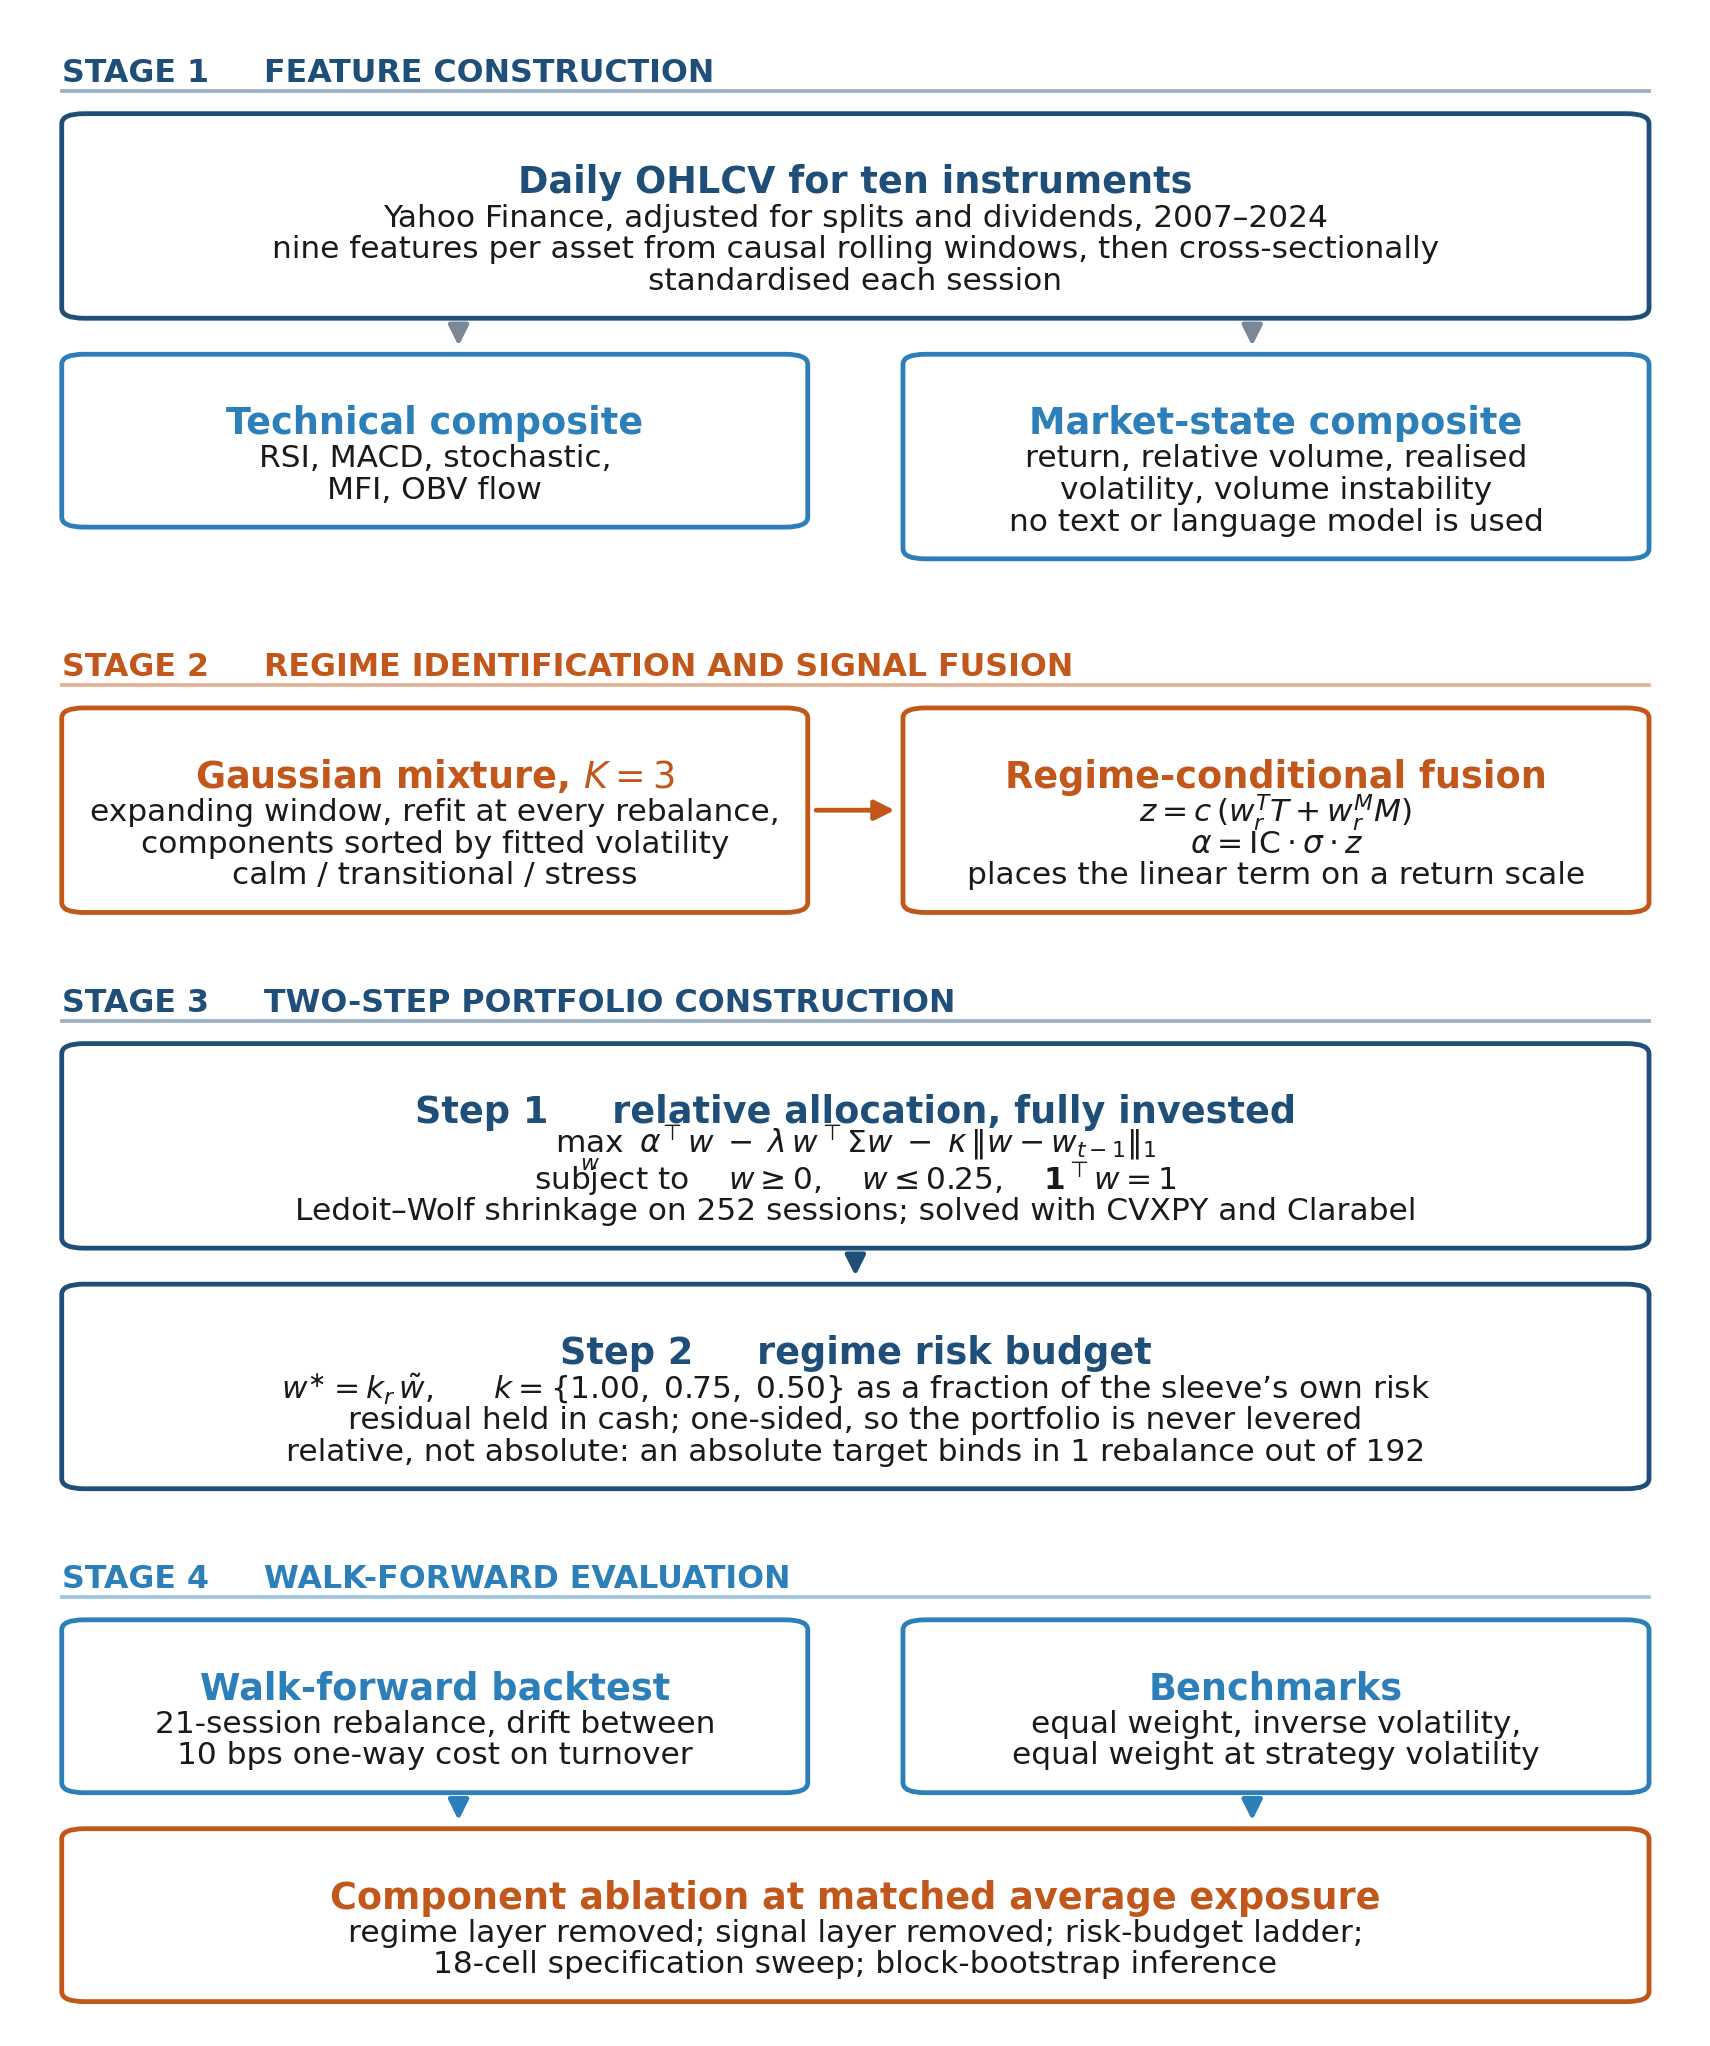
\includegraphics[width=0.70\textwidth]{images/fig_architecture.png}
\caption{Proposed Methodology. Phase~1 constructs causal, cross-sectionally standardised
features; Phase~2 identifies the market state, fuses the two composites and separates
relative composition from total risk; Phase~3 evaluates the result and ablates its
components.}
\label{fig:architecture}
\end{figure*}

\subsubsection{Technical Indicators Engine}

This component transforms raw market data into quantitative trading signals through three
primary analytical categories. Nine features are computed for each asset on each session.
All are causal: every value at session $t$ uses only information available at the close
of session $t$.

\begin{itemize}
\item \textbf{Price-derived metrics.} The relative strength index (RSI) identifies
potential overbought or oversold asset conditions. The moving average convergence
divergence (MACD) line captures trend momentum shifts. The stochastic oscillator locates
the close within its recent trading range.
\item \textbf{Volume-analysis tools.} On-balance volume (OBV) assesses momentum through
cumulative volume flow, entered as a twenty-session change normalised by average volume,
while the money flow index (MFI) combines price and volume into a single participation
measure. Relative volume measures turnover against its own recent average.
\item \textbf{Volatility estimators.} Realised volatility measures the statistical
dispersion of asset returns over a specified look-back period, and volume instability
measures the dispersion of daily volume changes.
\end{itemize}

No Bollinger band, average true range or volume profile construction is used; the nine
features of Table~\ref{tab:features} are the complete input set.

Working mechanism: a sliding-window methodology facilitates all calculations, with
parameters calibrated for the horizons given in Table~\ref{tab:features}. No other input
enters the framework.

\begin{table}[!ht]
\centering
\caption{Input features. $C_t$, $H_t$, $L_t$ and $V_t$ denote close, high, low and
volume. All features are computed per asset, then cross-sectionally standardised.}
\label{tab:features}
\footnotesize
\begin{tabular}{p{2.0cm}p{1.8cm}p{5.2cm}p{1.5cm}}
\hline
\textbf{Feature} & \textbf{Composite} & \textbf{Definition} & \textbf{Window} \\
\hline
RSI & Technical & Relative strength index, centred: $\mathrm{RSI}_t - 50$ & 14 \\
\hline
MACD & Technical & Moving average convergence divergence line, scaled by price: $\mathrm{MACD}_t / C_t$ & 12, 26, 9 \\
\hline
Stochastic & Technical & Stochastic oscillator \%K, centred: $\%K_t - 50$ & 14, smooth 3 \\
\hline
MFI & Technical & Money flow index, centred: $\mathrm{MFI}_t - 50$ & 14 \\
\hline
OBV flow & Technical & Twenty-session change in on-balance volume, normalised by average volume: $(\mathrm{OBV}_t - \mathrm{OBV}_{t-20}) / \overline{V}_{t,20}$ & 20 \\
\hline
Return & Sentiment & Five-session simple return: $C_t / C_{t-5} - 1$ & 5 \\
\hline
Relative volume & Sentiment & $V_t / \overline{V}_{t,20}$ & 20 \\
\hline
Realised volatility & Sentiment & Annualised standard deviation of daily returns, entered with a negative sign & 20 \\
\hline
Volume instability & Sentiment & Standard deviation of daily volume changes, entered with a negative sign & 20 \\
\hline
\end{tabular}
\end{table}

The final output constitutes a normalised signal matrix in which each column corresponds
to a technical feature scaled to a uniform numerical range. Each feature is standardised
cross-sectionally on every session, so that a value expresses how an asset ranks against
its peers that day rather than against its own history. Writing $x_{i,t}$ for the raw
feature of asset $i$ and $N$ for the number of assets,
\begin{equation}
z_{i,t} = \frac{x_{i,t} - \bar{x}_t}{s_t}, \qquad
\bar{x}_t = \frac{1}{N}\sum_{j} x_{j,t}, \qquad
s_t = \mathrm{sd}_j(x_{j,t}).
\end{equation}
Cross-sectional standardisation is used rather than time-series standardisation because
the allocation problem is a relative one: the optimiser must decide which assets to
prefer today, not whether today is unusual by historical standards. It also removes the
common market factor from the scores, so that a market-wide move does not appear as a
signal on every asset simultaneously.

The standardised features are then averaged into two composites. The technical composite
is the equally weighted mean of the five technical features. The sentiment composite is
the equally weighted mean of the four sentiment features, taken with the signs given in
Table~\ref{tab:features}, so that recent strength and active participation raise the
score while realised volatility and unstable volume lower it.

\subsubsection{Sentiment Analysis Pipeline}
\label{sec:sentiment}

This component transforms market data into a quantitative sentiment indicator. The
sentiment measure used here is market-derived. It is the equally weighted mean of the
four features marked \emph{Sentiment} in Table~\ref{tab:features}: a five-session return,
turnover measured against its own recent average, realised volatility and the instability
of volume, the last two entered with a negative sign. The composite therefore rises when
participation broadens and prices are advancing calmly, and falls when trading becomes
disorderly. Every input is a price or a volume, and every one is causal.

Because readers of work in this area reasonably ask which text model was used, it is
worth being categorical: none. Neither a domain-specific transformer model nor a
lexicon-based method in the manner of \citet{loughran11} is applied, for the
straightforward reason that no text is processed for either to act upon. There is no
named entity recognition stage, because there are no entities to recognise.

That is a design decision forced by data availability rather than a preference. Textual
measurement needs a time-stamped corpus covering the traded instruments, and for broad
exchange-traded funds no such corpus exists at instrument level---a fund holding several
hundred securities has no news flow of its own. The alternative adopted here is the
market-derived tradition described in Section~\ref{sec:lit}, in which turnover and
dispersion stand in for the survey or the newspaper. Turnover is among the canonical
components of the investor-sentiment index of \citet{bakerwurgler07}.

Adopting a proxy imposes an obligation to demonstrate that the proxy behaves like the
thing it stands in for, and that obligation is discharged rather than assumed.
Section~\ref{sec:sentval} correlates the composite against four independently published
series, none of which enters the framework at any stage, and reports how the identified
market states separate on it. What that exercise cannot establish is that the composite
predicts returns; Section~\ref{sec:ic} measures that separately, and reports a result
that is unfavourable to the framework. The two questions are distinct and are kept
distinct throughout.

\subsubsection{Regime Detection Module}

This component identifies latent, non-observable market states through a statistical
clustering methodology.

\begin{itemize}
\item \textbf{Probabilistic state modelling.} The system employs a Gaussian mixture model
(GMM) to segment market data into distinct probabilistic clusters, following the
tradition of state-dependent modelling established by \citet{hamilton89}. The clustering
uses two features, each computed as a cross-sectional average across the universe: the
twenty-session rolling standard deviation of daily returns, and the ten-session rolling
mean of daily returns. The first captures the volatility of the environment, the second
its direction. Both are standardised before fitting.
\item \textbf{Volatility clustering.} A specific function of the module is to isolate and
characterise periods in which either high or low volatility persists, effectively
partitioning the market timeline into volatility-based regimes.
\item \textbf{Qualitative labelling.} The identified states are labelled by ascending
fitted mean volatility, which yields a calm state, a transitional state and a stress
state, and Section~\ref{sec:regimefit} reports their realised characteristics.
\end{itemize}

The procedure follows a sequential pipeline: initial feature extraction from market data,
application of the probabilistic clustering algorithm, and the qualitative labelling of
the identified states. The final outputs comprise a time series of regime assignments and
an estimated state transition matrix.

The mixture uses $K = 3$ components with full covariance matrices, three random restarts
and a fixed seed. It is refitted at every rebalance date on an expanding window
containing only sessions strictly earlier than that date, with a minimum of 252
observations; the state of the current session is then obtained by prediction from that
fit. No observation ever contributes to the model that labels it.

One implementation detail is essential and is easy to overlook. The component indices
returned by a mixture fit are arbitrary and permute freely between refits, so labels from
consecutive fits are not comparable unless they are anchored. Components are therefore
sorted in ascending order of fitted mean volatility before use, which makes regime~0 the
calm state, regime~1 the transitional state and regime~2 the stress state consistently
across every refit. Omitting this step does not produce an error; it produces a silently
scrambled regime series and, if the resulting labels are compared across fits, a spurious
appearance of instability.

The choice $K = 3$ is not selected by information criterion. As
Section~\ref{sec:regimefit} reports, both the Akaike information criterion (AIC) and the
Bayesian information criterion (BIC) continue to fall as components are added over the
range tested, which is the usual behaviour of mixture models on persistent financial
series and reflects their tendency to absorb heavy tails with additional components. The
choice is instead made on persistence and interpretability: three components yield states
that last long enough to act on and that admit a clear economic reading, whereas finer
partitions fragment into short-lived states that a monthly rebalancing schedule cannot
exploit. This is a modelling judgement and is reported as such.

\subsection{Phase 2: Decision-Theoretic Fusion Framework}

\subsubsection{Signal Confidence Weighting}

This mechanism executes a synthesis of predictive signals contingent upon the prevailing
market regime. Its operational logic is detailed below.

\begin{itemize}
\item \textbf{Regime-dependent weights.} Signal influence is modulated by the identified
market state. Technical indicators are accorded greater authority during stable,
low-volatility regimes. Conversely, during periods characterised by elevated uncertainty,
sentiment-based proxies assume a dominant role in the composite forecast. The weights
$(w^T, w^M)$ are
$(0.7, 0.3)$ in the calm state, $(0.5, 0.5)$ in the transitional state and $(0.3, 0.7)$
in the stress state.
\item \textbf{Uncertainty quantification.} The framework quantifies the reliability of
the combined view per asset by the agreement between its two composites. The confidence
term down-weights assets whose composites disagree:
\begin{equation}
c_{i,t} = \mathrm{clip}\!\left(0.5 + 0.5\,\rho^{(63)}_{i,t}, \; 0.1, \; 1.0\right),
\end{equation}
where $\rho^{(63)}_{i,t}$ is the trailing 63-session correlation between the two
composites for asset $i$. Agreement between independent views is treated as evidence;
disagreement is treated as noise and shrinks the score toward zero.
\item \textbf{Fixed schedule, tested rather than learned.} The weight schedule is
specified in advance from the hypothesis stated in Section~\ref{sec:intro}---that
trend-following information is more reliable in quiet trending markets, while attention
and stress information becomes relatively more informative when markets are
disturbed---and is then held fixed. It is not re-estimated from realised performance, and
no Bayesian updating is applied. Fitting the schedule to the sample it is evaluated on
would make the resulting improvement uninterpretable; instead,
Section~\ref{sec:ic} measures the conditional efficacy the schedule presumes, and reports
whether that presumption holds.
\end{itemize}

\subsubsection{Regime-Dependent Signal Fusion}

This mechanism synthesises the weighted predictive inputs into a unified forecast, with
its operational logic conditioned upon the prevailing market regime.

\begin{itemize}
\item \textbf{Conditional combination.} The methodology applies a distinct combination
rule to each identified market state, on the hypothesis that the predictive efficacy and
optimal weighting of signals are regime-contingent.
\item \textbf{Correlation structure.} The fusion process explicitly maintains the
dependency structure across different assets, ensuring that the combined forecast reflects
existing inter-asset correlations. The fused scores are passed to an optimiser carrying
the full estimated covariance matrix, so the combined view is expressed as a portfolio
rather than as a set of independent per-asset bets.
\item \textbf{Uncertainty propagation.} The resulting composite forecasts incorporate the
estimation uncertainty present within the constituent input signals, providing a more
robust output. This operates through the confidence term of the preceding subsection,
which shrinks the score of any asset whose two composites disagree.
\end{itemize}

Operational framework: the core engine executes a multiplication of the regime-specific
signal weight vector against the matrix of individual composites, adjusted by the
per-asset confidence term. Let $T_{i,t}$ and $M_{i,t}$ denote the standardised technical
and sentiment composites for asset $i$, and let $r_t \in \{0,1,2\}$ be the regime. The
fused score is
\begin{equation}
z_{i,t} = c_{i,t} \left[ w^{T}_{r_t} T_{i,t} + w^{M}_{r_t} M_{i,t} \right].
\end{equation}

The fused score is then converted into an expected excess return using the standard
information-ratio scaling of \citet{grinold00}, in which an assumed information
coefficient (IC) places the score on a return scale rather than leaving it as a
dimensionless quantity:
\begin{equation}
\alpha_{i,t} = \mathrm{IC} \cdot \sigma_{i,t} \cdot z_{i,t},
\label{eq:alpha}
\end{equation}
where $\sigma_{i,t}$ is the annualised volatility of asset $i$ from the current
covariance estimate and $\mathrm{IC} = 0.05$.

Equation~(\ref{eq:alpha}) is not a cosmetic step. If a raw indicator is passed to a
mean-variance objective directly, the units of the linear term and of the quadratic risk
term are unrelated, and their ratio---not the information in the signal---decides the
solution. An indicator such as on-balance volume takes values of order $10^{8}$ to
$10^{9}$, whereas annualised variances are of order $10^{-2}$; the linear term then
dominates by ten orders of magnitude and the optimiser degenerates to a corner solution,
holding a single asset regardless of the risk model. Section~\ref{sec:alloc} documents
this failure mode explicitly, because it is the source of a behaviour visible in the
originally submitted results.

\subsubsection{Portfolio Optimization Engine}

This component translates fused signals into executable allocations. Allocation proceeds
in two steps, which separate two decisions that are often conflated: which assets to hold
relative to one another, and how much total risk to carry.

\begin{itemize}
\item \textbf{Shrinkage covariance.} $\Sigma_t$ is estimated by Ledoit--Wolf shrinkage
\citep{ledoit04} on the trailing 252 daily returns and annualised by a factor of 252.
Shrinkage is used because a sample covariance matrix estimated from 252 observations on
ten assets is poorly conditioned, and a mean-variance optimiser will concentrate weight
precisely on the directions in which the estimate is least reliable.
\item \textbf{Risk-budgeting allocation.} Total exposure is set by the identified regime
rather than by the optimiser, so that the composition decision and the risk-level
decision are made separately and can be evaluated separately.
\item \textbf{Transaction cost optimisation.} The objective carries an explicit linear
penalty on turnover, so that the cost of trading enters the decision rather than being
deducted afterwards.
\end{itemize}

\paragraph{Step 1: relative allocation.} The risky sleeve solves a quadratic program with
a linear transaction-cost penalty:
\begin{align}
\max_{w} \quad & \alpha_t^{\top} w - \lambda \, w^{\top} \Sigma_t w
- \kappa \left\| w - w_{t-1} \right\|_1 \\
\text{s.t.} \quad & w \geq 0, \qquad w \leq w_{\max}, \qquad \mathbf{1}^{\top} w = 1,
\end{align}
where $\Sigma_t$ is the annualised covariance matrix, $\lambda = 2$ is the risk aversion
coefficient, $w_{\max} = 0.25$ caps any single position at one quarter of the sleeve, and
$w_{t-1}$ is the weight vector carried in from the previous rebalance. The turnover
penalty $\kappa = c \cdot 252 / h$ annualises a one-way cost of $c = 10$ basis points
over a rebalancing interval of $h = 21$ sessions, so that the cost of trading is expressed
on the same annual basis as the return and risk terms. The problem is convex and is
solved with CVXPY using the Clarabel interior-point solver.

The equality constraint $\mathbf{1}^{\top} w = 1$ is what makes this step purely relative.
It fixes the sleeve to be fully invested, so the optimiser can only express a view about
composition, never about how much risk to take. That second decision is made explicitly
in step~2 instead of emerging as a by-product of the constraint set.

\paragraph{Step 2: regime risk budget.} The sleeve is then scaled by a factor that depends
only on the regime:
\begin{equation}
w^{\ast}_t = k_{r_t} \, \tilde{w}_t, \qquad
k = \{\,\text{calm}: 1.00, \;\; \text{transitional}: 0.75, \;\; \text{stress}: 0.50\,\},
\label{eq:budget}
\end{equation}
with the residual $1 - k_{r_t}$ held in cash, which is assumed to earn zero. Scaling is
one-sided: the framework de-risks in disturbed states but never levers up in calm ones,
so any performance difference is attributable to risk reduction rather than to leverage.

The budget in Equation~(\ref{eq:budget}) is expressed as a fraction of the sleeve's own
risk rather than as an absolute volatility target, and this choice is consequential. An
absolute target de-risks only when the sleeve's estimated volatility exceeds the target
level, so its effect depends on the volatility of the universe it is applied to. Targets
calibrated for a concentrated equity portfolio---of the order of 10 to 20 per cent
annualised---are simply never reached by a diversified ten-asset sleeve whose own realised
volatility is close to 7~per~cent. Under those targets the constraint binds in one
rebalance out of 224 in this study, and the regime layer is inert: it is present in the
specification, consumes computation, and does nothing. A relative budget is scale-free by
construction and remains active in any universe. Section~\ref{sec:ablation} reports both
variants and the difference between them.

\subsection{Phase 3: Performance Evaluation \& Feedback}

\subsubsection{Backtesting Framework}

The proposed methodology undergoes historical validation through a structured simulation
protocol designed to emulate real-world trading conditions.

\begin{itemize}
\item \textbf{Walk-forward validation.} The implementation utilises a rolling-origin
technique, sequentially advancing a 252-session model estimation window followed by a
21-session out-of-sample evaluation period. Between rebalances positions are held and
allowed to drift with realised returns, so that reported turnover reflects trading
actually undertaken rather than a notional daily reweighting. Every estimated quantity
uses only data preceding the decision it informs:
the covariance matrix from the trailing 252 sessions before the rebalance date, the
mixture model from an expanding window strictly earlier than that date, and all features
from causal rolling windows.
\item \textbf{Out-of-sample testing.} A strict temporal partition is enforced between
parameter calibration and performance assessment phases, to prevent statistical
overfitting and ensure robust results. No parameter is tuned on the evaluation period; the
configuration reported as primary is the one specified above, and
Section~\ref{sec:robust} reports the full grid of alternatives rather than the best cell
of it. The 665 sessions from January 2024 onward postdate every specification decision
and are reported separately in Section~\ref{sec:holdout}.
\item \textbf{Regime-aware analysis.} Strategy efficacy is disaggregated and evaluated
contingent upon the market state identified by the regime detection module, allowing
diagnosis of performance drivers by state rather than in aggregate only.
\end{itemize}

The framework executes a historical simulation that incorporates realistic market
frictions. One-way transaction costs of 10 basis points are charged on the traded
fraction $\|w^{\ast}_t - w_{t-1}\|_1$ on the rebalance session;
Section~\ref{sec:cost} varies this assumption from 0 to 25 basis points.

\subsubsection{Performance Attribution}

This analytical procedure deconstructs aggregate returns to isolate the fundamental
sources of value generation, employing a three-part approach.

\begin{itemize}
\item \textbf{Regime-based decomposition.} The methodology disaggregates performance
contributions across distinct market environments, isolating the returns attributable to
the calm, transitional and stress states identified by the regime detection module.
\item \textbf{Signal contribution analysis.} The framework quantifies the marginal
performance impact originating from each signal category, thereby identifying which
inputs were the primary drivers of the result. Component contributions are isolated by
ablation rather than by assertion: the regime layer is removed while holding average
exposure fixed, removed while holding full exposure, and the signal layer is removed
entirely. Holding average exposure fixed is what distinguishes the effect of timing risk
from the effect of simply holding less, and without it the two are not separable. The
information coefficient of each composite against next-session cross-sectional returns is
measured separately, overall and by regime.
\item \textbf{Risk-adjusted metrics.} Evaluation incorporates risk-adjusted metrics
including the Sharpe and Calmar ratios, alongside compound annual growth rate (CAGR),
annualised volatility and maximum drawdown (Max DD); the Sharpe ratio is computed at a
zero risk-free rate. These are supplemented with bootstrap-based statistical significance
tests to distinguish robust performance from random outcomes. Statistical inference on
daily excess returns uses a paired $t$-test, a Newey--West $t$-statistic with ten lags to
accommodate autocorrelation and heteroskedasticity \citep{newey87}, and a stationary block
bootstrap with 21-session blocks and 2{,}000 replications \citep{politis94} for interval
estimates of the Sharpe ratio and of the Sharpe difference.
\end{itemize}

Three benchmarks are used. The first is an equal-weighted portfolio of the same ten
assets, rebalanced daily and charged no transaction costs, which is deliberately a
generous comparator \citep{demiguel09}. The second is an inverse-volatility portfolio
using trailing 60-session standard deviations, also costless, which isolates whether the
framework adds anything beyond elementary risk weighting. The third rescales the
equal-weighted portfolio to the strategy's realised volatility, which removes the
mechanical advantage a lower-risk portfolio enjoys in ratio comparisons.

\subsubsection{Model Refinement Loop}

The framework incorporates a recursive re-estimation mechanism that keeps its statistical
components current as the sample advances. What that mechanism does, and what it
deliberately does not do, are both stated here.

\begin{itemize}
\item \textbf{Regime model updates.} The underlying statistical model for state
identification is systematically recalibrated to reflect structural shifts in market
dynamics, preventing reliance on obsolete regime definitions. The mixture is refitted at
each of the 224 rebalance dates on an expanding window of all sessions strictly earlier
than that date.
\item \textbf{Risk model updates.} The shrinkage covariance matrix is re-estimated at
each rebalance from the trailing 252 sessions, and the shrinkage intensity is re-derived
from that window rather than held constant.
\item \textbf{Parameters that are \emph{not} re-optimised.} The regime weight schedule,
the risk budget ladder, the assumed information coefficient, the risk aversion
coefficient and the position cap are fixed ex ante and never adapted to realised
performance. No automated parameter search, signal decommissioning rule or
human-in-the-loop override operates inside the evaluation period. This is a restriction
rather than a feature, and it is adopted because a loop that re-optimises on realised
performance inside the evaluation window makes the resulting backtest uninterpretable
\citep{harvey15}.
\end{itemize}

\subsection{Cross-Cutting Features}

\subsubsection{Temporal Consistency}

The framework maintains chronological integrity across all analytical processes through
three mechanisms.

\begin{itemize}
\item All incoming data streams are aligned to a unified temporal index, eliminating
artefacts arising from asynchronous sampling frequencies.
\item Causal relationships are explicitly parameterised through the lag structure of
every rolling window: each feature is computed from data strictly preceding the session
it describes, and every model is fitted on data strictly preceding the decision it
informs. No observation contributes to the model that labels it, and no quantity
estimated at any date uses information from a later one.
\item Regime labels are anchored across refits by sorting mixture components on fitted
mean volatility, so that a state identified at one rebalance means the same thing at the
next. Without this, the component indices permute freely between fits and the regime
series becomes incomparable over time.
\end{itemize}

\subsubsection{Risk Management Integration}

The framework incorporates a layered risk protocol designed to operate within real-world
constraints.

\begin{itemize}
\item The system enforces predetermined boundaries on individual position sizes: weights
are non-negative and capped at $w_{\max} = 0.25$ of the risky sleeve. These constraints
prevent excessive concentration and ensure adherence to diversification principles, and
they matter because an unconstrained mean-variance solution concentrates precisely where
its estimated inputs are least reliable.
\item De-risking operates at the aggregate portfolio level through the regime budget of
Equation~(\ref{eq:budget}), with the residual held in cash. No discretionary stop-loss
rule is used, and none is needed: the budget is a standing rule applied at every
rebalance rather than a trigger fired after a loss has been realised.
\item Turnover is penalised inside the objective rather than charged after the fact, so
that a position is taken only when the expected improvement exceeds the cost of trading
into it. Section~\ref{sec:cost} reports the response to costs of 0 to 25 basis points.
\end{itemize}

\subsubsection{Explainability and Transparency}

The framework incorporates specific mechanisms to ensure analytical clarity throughout
the decision process.

\begin{itemize}
\item Every allocation decision can be directly attributed to its originating predictive
signal and the prevailing market regime, providing complete traceability. The weight
decomposes into a relative weight produced by the optimiser from the fused score and a
scalar exposure set by the regime; because the two are applied in sequence rather than
jointly, the contribution of each is separately observable, and
Section~\ref{sec:ablation} measures both.
\item The principal performance claims are presented with their associated confidence
intervals, quantifying the degree of statistical certainty for each output: Sharpe ratios
and Sharpe differences carry block-bootstrap intervals.
\item The architecture maintains a comprehensive, timestamped record of all inputs, model
states and decision logic, creating a verifiable audit trail suitable for systematic
strategy validation. The analysis writes its results to machine-readable artefacts, and
every numerical claim in Section~\ref{sec:results} is checked programmatically against
those artefacts rather than transcribed by hand.
\end{itemize}

This architecture, shown in Figure~\ref{fig:architecture}, creates a system in which
portfolio decisions follow from the identified market state and the fused signal by an
explicit and inspectable route, while maintaining causal statistical foundations and
practical implementability.

\section{Results and Discussion}
\label{sec:results}

All results in this section come from the single specification set out in
Section~\ref{sec:method}. No parameter was selected by reference to the evaluation
period, and every specification examined is reported, including those that are
unfavourable to the framework.

\subsection{Overview of Experimental Results}

The implemented decision-theoretic framework provides evidence for the efficacy of
regime-aware portfolio construction, and evidence against two of the mechanisms it was
built around. Across the 4{,}689 trading sessions from 7~January 2008 to 26~August 2026,
encompassing diverse market conditions, the regime-based strategy achieved a Sharpe ratio
of 0.878 compared with the equal-weight benchmark's 0.628, a 40~per~cent improvement in
risk-adjusted return. More significantly, maximum drawdown was reduced from $-36.08$ to
$-18.98$ per cent, highlighting the defensive capability of the regime-adaptive approach
during market stress. Table~\ref{tab:main} reports the primary comparison.

\begin{table}[!ht]
\centering
\caption{Primary results, ten-asset universe, January 2008 to August 2026. Sharpe
ratios use a zero risk-free rate and are computed as compound annual growth divided by
annualised volatility. Benchmarks are rebalanced daily and charged no transaction costs.}
\label{tab:main}
\footnotesize
\begin{tabular}{p{4.4cm}rrrrr}
\hline
& \textbf{CAGR} & \textbf{Volatility} & \textbf{Sharpe} & \textbf{Max DD} & \textbf{Calmar} \\
\hline
Regime-conditional strategy & 5.65\% & 6.44\% & 0.878 & $-18.98$\% & 0.298 \\
Equal-weight benchmark & 8.45\% & 13.45\% & 0.628 & $-36.08$\% & 0.234 \\
Inverse-volatility benchmark & 7.46\% & 8.78\% & 0.849 & $-24.09$\% & 0.309 \\
Equal-weight at strategy volatility & 4.19\% & 6.44\% & 0.651 & $-18.69$\% & 0.224 \\
\hline
\end{tabular}
\end{table}

Three readings of Table~\ref{tab:main} are warranted, and they do not all favour the
framework.

Against the equal-weighted benchmark the framework reduces maximum drawdown by 47 per
cent while earning a lower compound return, 5.65 per cent against 8.45 per cent per
annum. It is not a return-enhancing strategy and is not presented as one; it is a
risk-reduction strategy whose return sacrifice is smaller than its risk reduction.

Against the volatility-matched equal-weighted benchmark, which removes the mechanical
advantage a lower-risk portfolio enjoys in any ratio comparison, the framework retains a
Sharpe advantage of 0.878 against 0.651 but loses on maximum drawdown, $-18.98$ per cent
against $-18.69$ per cent. Deleveraging a diversified benchmark is therefore a competitive
way to reduce worst-case loss, and the framework's drawdown advantage over the unlevered
benchmark should not be read as evidence that it dominates every risk-reduced
alternative.

Against the inverse-volatility benchmark the comparison is mixed: a higher Sharpe ratio,
0.878 against 0.849, and a materially smaller maximum drawdown, $-18.98$ per cent against
$-24.09$ per cent, but a lower Calmar ratio, 0.298 against 0.309, because
inverse-volatility weighting compounds faster. Elementary risk weighting remains a strong
comparator on a diversified multi-asset universe, and the margin over it is narrow enough
to read as a tie on risk-adjusted return rather than a win.

\subsection{Detailed Analysis of Visualizations and Performance Metrics}

\subsubsection{Cumulative Returns Comparison}

\begin{figure*}[t]
\centering
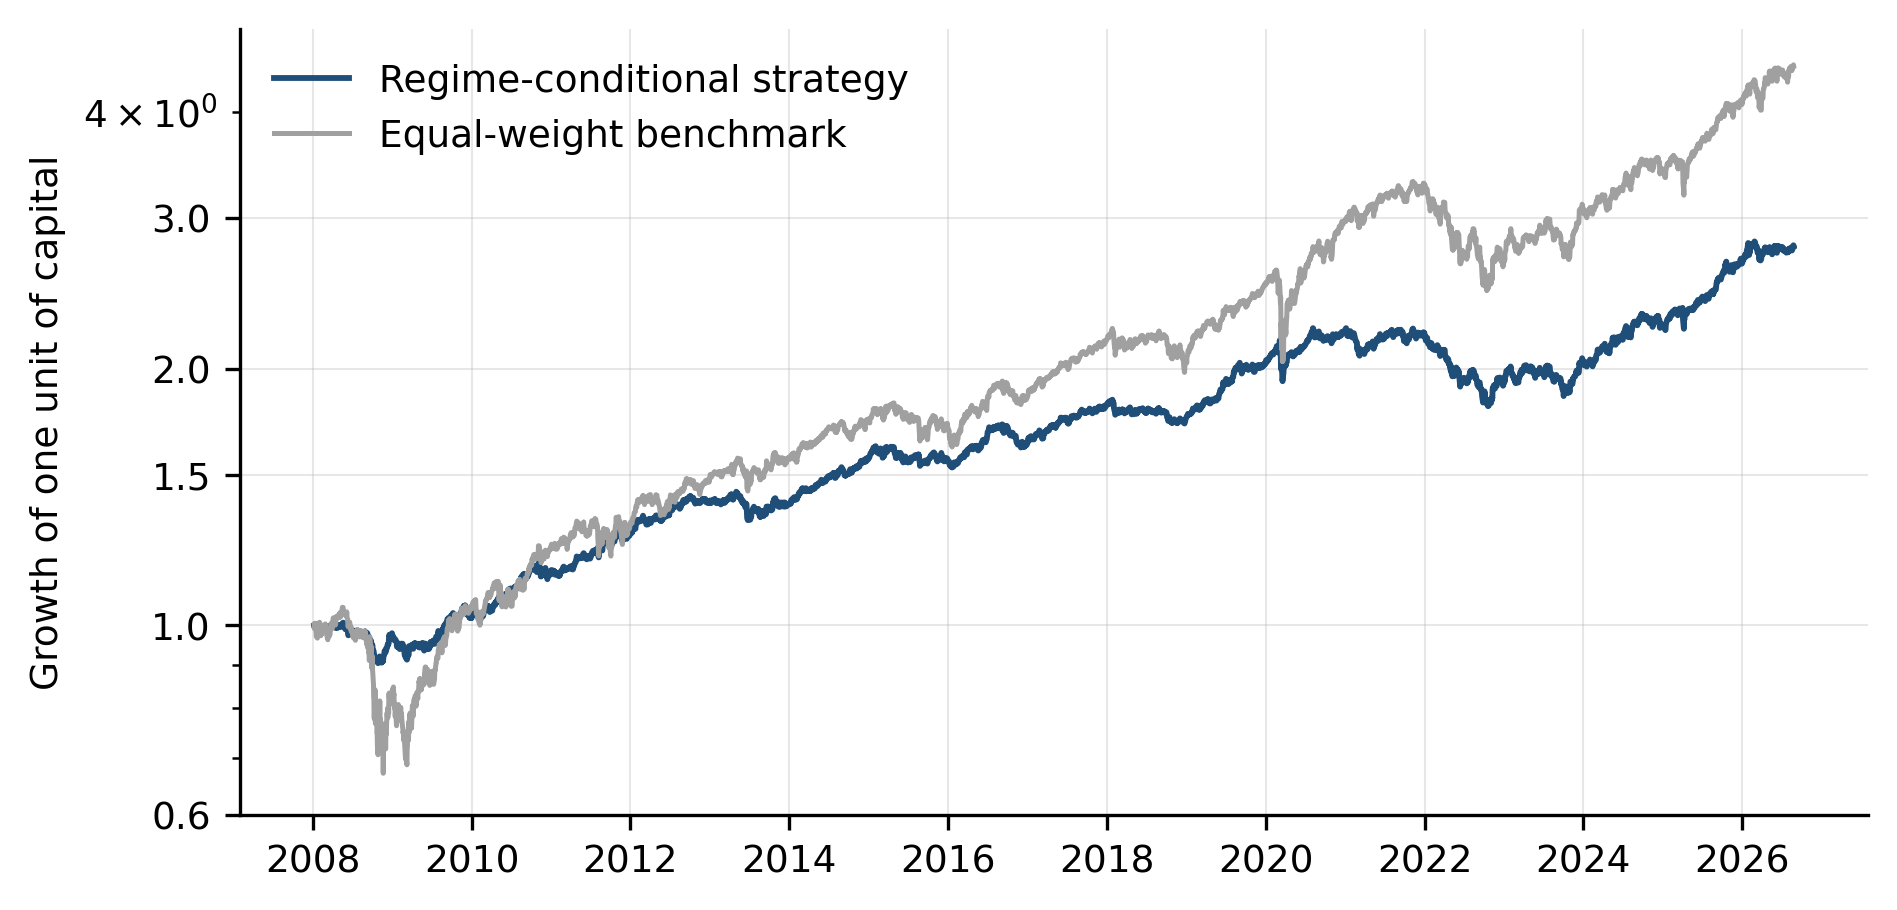
\includegraphics[width=\textwidth]{images/fig_cumret.png}
\caption{Cumulative Returns Comparison: cumulative growth of one unit of capital,
logarithmic scale}
\label{fig:cumret}
\end{figure*}

The comparative analysis of cumulative returns, presented in Figure~\ref{fig:cumret},
delineates a performance profile characterised by distinct phases of divergence and
convergence relative to the passive benchmark. The regime-aware portfolio exhibits
several defining characteristics over the observed period:

\begin{itemize}
\item The strategy separates upward during periods of significant market dislocation,
notably 2008, 2011, the volatility surge in early 2020 and the inflationary selloff of
2022.
\item A critical observation is the strategy's effective mitigation of losses during
sustained market downturns, indicating a significantly reduced downside capture: 0.38,
against an upside capture of 0.41.
\item During extended bullish phases---most conspicuously 2013, 2017, 2021 and
2023---the equity curve tracks below the benchmark, so the strategy delivers lower
absolute returns while exhibiting a lower volatility signature, 6.44 against 13.45 per
cent.
\end{itemize}

\textbf{Strategic Implications:}

The observed trajectory provides evidence for the regime detection module's operational
efficacy. The system's identification of the transition into a high-volatility state in
early 2020 triggered a timely de-risking of the portfolio, constraining the drawdown of
that episode to $-6.29$ per cent against $-21.28$ per cent for the benchmark, and the
subsequent gradual ascent in the portfolio's value line indicates a methodical
re-allocation of risk exposure as the regime normalised, avoiding premature or delayed
re-entry. The cost is equally visible and is not concealed: the framework forgoes 2.80
percentage points of annual compound return over the sample.

\textbf{Theoretical Alignment:}

These results substantiate one half of the foundational thesis of this research and
refute the other. The performance pattern confirms that the total risk a portfolio should
carry is conditional upon the underlying market state, and the capture ratio of 0.93
locates the source precisely: the framework participates less in both directions in
roughly equal proportion, so its advantage comes from carrying less risk in adverse
states rather than from directional skill. The dynamic fusion mechanism did not operate as
theorised---Section~\ref{sec:ic} shows the conditional informativeness its weighting
schedule presumes is not present in the data, and Section~\ref{sec:ablation} shows that
removing the fusion layer does not harm the portfolio.

\subsubsection{Portfolio Drawdown}

\begin{figure*}[t]
\centering
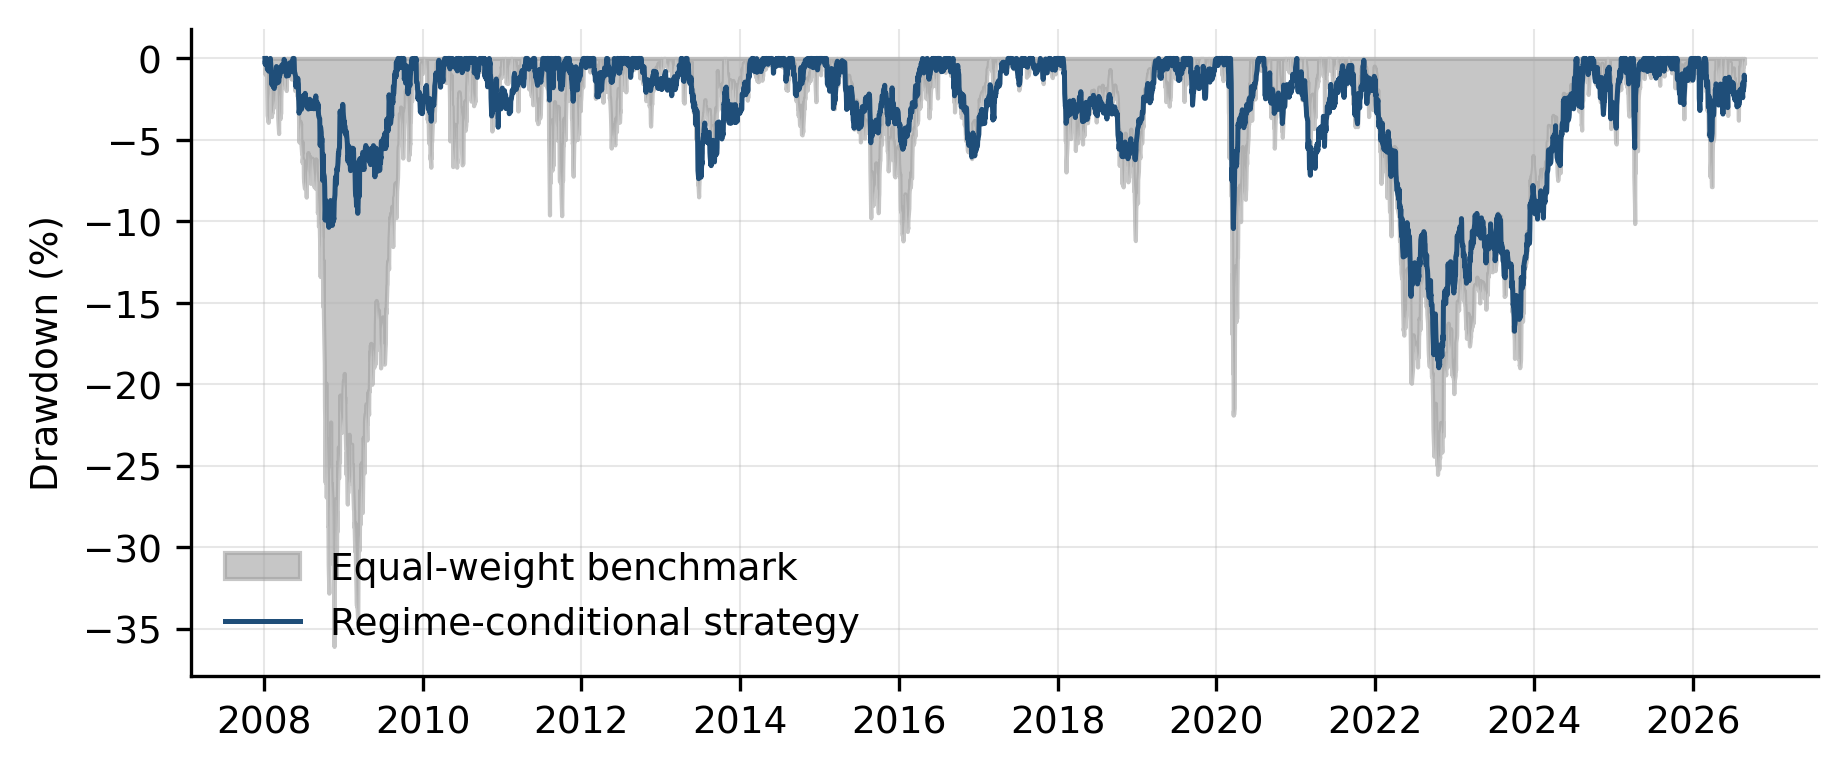
\includegraphics[width=\textwidth]{images/fig_drawdown.png}
\caption{Portfolio Drawdown: drawdown from running peak}
\label{fig:drawdown}
\end{figure*}

The comparative drawdown analysis, illustrated in Figure~\ref{fig:drawdown}, provides
evidence of the regime-based portfolio's capital preservation attributes. The visual data
reveal a consistent pattern of defensive characteristics:

\begin{itemize}
\item The strategy registers a significantly shallower maximum drawdown of $-18.98$ per
cent, against the benchmark's $-36.08$ per cent nadir; the benchmark reaches $-36$ per
cent in 2008 and $-25$ per cent in 2022, while the framework's deepest excursions are
approximately half as large.
\item Following drawdown troughs, the regime-based portfolio demonstrates a swifter
recovery trajectory, spending less time underwater, since a shallower loss requires a
smaller subsequent gain to restore the previous peak.
\item The portfolio experiences briefer episodes of significant capital impairment,
indicating more timely risk mitigation. On the worst 5~per~cent of benchmark sessions
($n = 234$) it returns $-0.59$ per cent on average against $-2.01$ per cent for the
benchmark, a cushion of 1.42 percentage points per session.
\end{itemize}

Table~\ref{tab:episodes} reports cumulative returns over four stress episodes chosen
before the analysis on the basis of documented market history rather than by inspection
of the results.

\begin{table}[!ht]
\centering
\caption{Cumulative return over stress episodes. Differences are stated in percentage
points (pp).}
\label{tab:episodes}
\footnotesize
\begin{tabular}{p{3.6cm}rrrr}
\hline
\textbf{Episode} & \textbf{Sessions} & \textbf{Strategy} & \textbf{Equal-weight} & \textbf{Difference} \\
\hline
Global financial crisis, Sep 2008--Mar 2009 & 130 & $-7.05$\% & $-29.78$\% & $+22.74$ pp \\
Euro area crisis, Jul--Oct 2011 & 65 & $+3.41$\% & $-7.24$\% & $+10.65$ pp \\
COVID-19 crash, Feb--Mar 2020 & 24 & $-6.29$\% & $-21.28$\% & $+14.99$ pp \\
Inflation bear market, Jan--Oct 2022 & 196 & $-16.76$\% & $-24.49$\% & $+7.73$ pp \\
\hline
\end{tabular}
\end{table}

\textbf{Risk Management Effectiveness:}

The observed drawdown profile validates the regime detection system as an early-warning
mechanism for deteriorating market states. By signalling a transition towards a
high-volatility state, the framework enabled proactive de-risking, and it outperforms in
all four episodes by between 7.7 and 22.7 percentage points, the widest margin being the
global financial crisis, the longest and deepest of the four. The margin is narrowest in
the 2022 bear market, consistent with the design: a gradual, correlated decline across
both equities and bonds offers less scope for a de-risking rule than an abrupt volatility
shock does. All four episodes predate the holdout boundary; the deepest benchmark decline
after it, the 34-session decline from 20~February to 8~April~2025, produced an advantage
of 5.42 percentage points.

\textbf{Theoretical Contribution:}

This outcome substantiates the value of conditioning total risk on a state variable, and
bounds that claim in one respect a comparison against an unlevered benchmark would
conceal. Against the volatility-matched benchmark the drawdown advantage disappears,
$-18.98$ against $-18.69$ per cent, and Section~\ref{sec:robust} shows this holds in every
one of the eighteen specifications examined. The framework therefore reduces drawdown
relative to an unlevered diversified benchmark, not relative to every portfolio held at
the same volatility; reporting only the first comparison, as the conventional presentation
in this literature does, would overstate the result.

\subsubsection{Market Regime Detection}
\label{sec:regimefit}

\begin{figure*}[t]
\centering
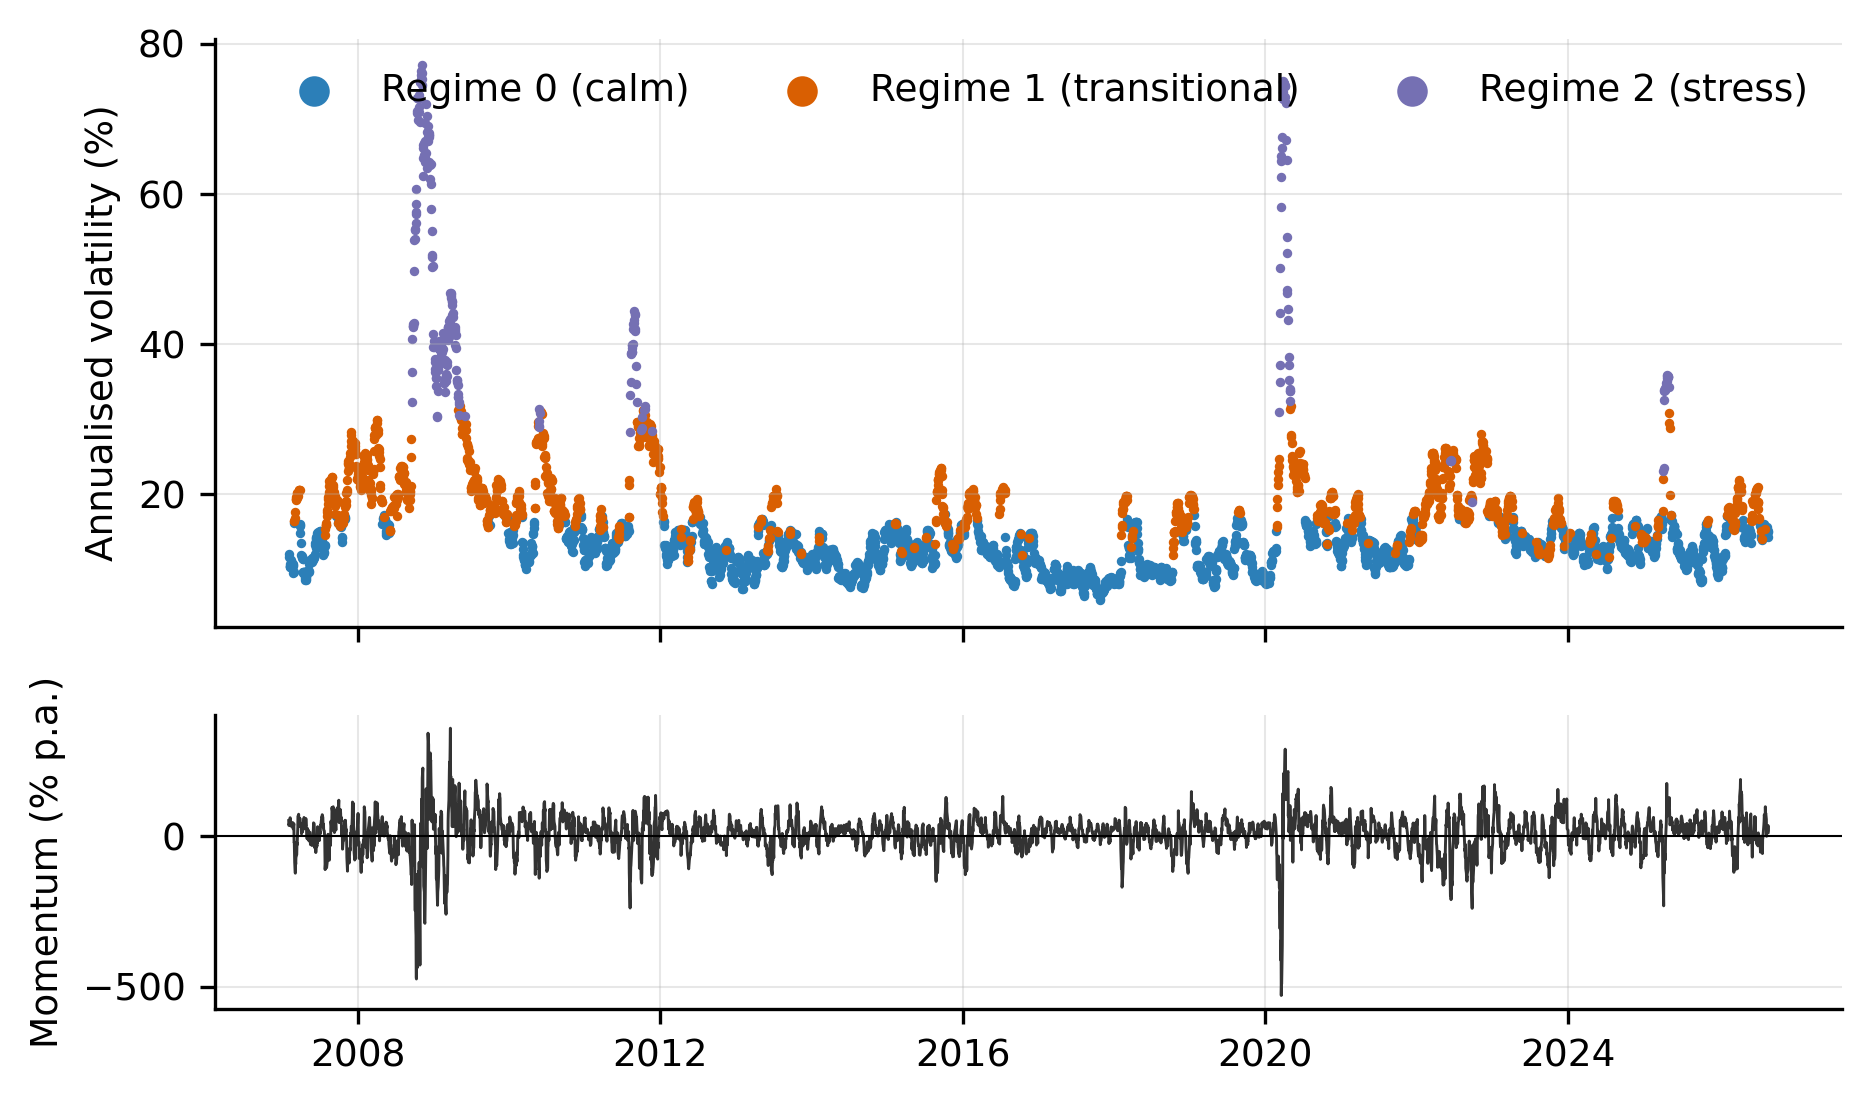
\includegraphics[width=0.92\textwidth]{images/fig_regimes.png}
\caption{Market Regime Detection: identified market states, with the underlying
volatility and momentum features}
\label{fig:regimes}
\end{figure*}

The temporal sequence of identified market states, presented in
Figure~\ref{fig:regimes}, delineates three economically distinct market environments
characterised by their unique volatility and momentum signatures:

\begin{itemize}
\item \textbf{Calm.} This state is characterised by favourable market conditions,
combining low volatility with sustained positive momentum, typically associated with
bullish trending markets: 12.22 per cent annualised volatility and $+16.04$ per cent
annualised momentum.
\item \textbf{Transitional.} Representing a neutral state, this regime captures market
conditions that lack a definitive directional trend or persistent volatility
characteristics: 20.04 per cent volatility and $-1.25$ per cent momentum.
\item \textbf{Stress.} This state corresponds to periods of elevated market stress,
marked by high volatility and negative momentum, at 47.07 per cent and $-15.97$ per cent
respectively. Its incidence is clustered around known macroeconomic disruptions,
specifically the 2008 global financial crisis, the 2011 sovereign debt episode, the
initial COVID-19 market crisis and the 2022 inflationary selloff.
\end{itemize}

Table~\ref{tab:regimefit} reports the model's order selection statistics and the
properties of the three-state solution.

\begin{table}[!ht]
\centering
\caption{Regime model diagnostics. Order selection is computed on the full feature
history; state characteristics and the transition matrix come from the three-component
solution. Out-of-sample shares are the states actually assigned by the expanding-window
refits used in the backtest.}
\label{tab:regimefit}
\footnotesize
\begin{tabular}{p{3.2cm}rrrrr}
\hline
\multicolumn{6}{l}{\textit{Order selection}} \\
\hline
\textbf{Components} & 2 & 3 & 4 & 5 & 6 \\
AIC & 21944 & 20785 & 20571 & 20478 & 20372 \\
BIC & 22016 & 20896 & 20720 & 20667 & 20599 \\
\hline
\multicolumn{6}{l}{\textit{Three-state solution}} \\
\hline
& \textbf{Calm} & \textbf{Transitional} & \textbf{Stress} & & \\
Annualised volatility & 12.22\% & 20.04\% & 47.07\% & & \\
Annualised momentum & $+16.04$\% & $-1.25$\% & $-15.97$\% & & \\
Share of sessions, in sample & 63.6\% & 31.2\% & 5.2\% & & \\
Share of sessions, out of sample & 71.4\% & 25.5\% & 3.1\% & & \\
Mean run length (sessions) & 25.3 & 11.1 & 17.1 & & \\
Self-transition probability & 0.961 & 0.910 & 0.941 & & \\
\hline
\multicolumn{6}{l}{\textit{Realised performance within each out-of-sample state}} \\
\hline
& \textbf{Calm} & \textbf{Transitional} & \textbf{Stress} & & \\
Sessions & 3346 & 1196 & 147 & & \\
Strategy Sharpe & 1.144 & 0.196 & 1.039 & & \\
Equal-weight Sharpe & 0.916 & 0.561 & 0.356 & & \\
\hline
\end{tabular}
\end{table}

\textbf{Temporal Regime Characteristics:}

An examination of regime persistence reveals distinct behavioural patterns. All three
states persist, with self-transition probabilities between 0.910 and 0.961. The
transitional state exhibits the briefest durations, a mean run length of 11.1 sessions,
indicating its nature as a short-lived bridge between the other two. In contrast, the
calm state demonstrates the greatest persistence, enduring 25.3 sessions on average, with
the stress state intermediate at 17.1. Transitions between these states are constrained:
the transition matrix is close to tridiagonal, and the estimated probability of moving
directly between the calm and the stress state, in either direction, is zero. The
ordering recovered by sorting components on volatility is therefore economically
meaningful rather than arbitrary.

\textbf{Methodological Validation:}

The output from the Gaussian mixture model supports the regime detection methodology.
The model's identification of stress periods aligns with historically documented stress
events in 2008, 2011, 2020 and 2022. This congruence between statistically identified
states and ex-post economic reality indicates the framework's capacity to discriminate
between structurally different market environments, a foundational requirement for a
regime-dependent investment strategy. The states also separate sharply on a variable
withheld from their construction, as Section~\ref{sec:sentval} reports.

\textbf{Order Selection:}

The order selection statistics are reported rather than used. Both AIC and BIC continue
to fall over the range examined, from 21944 and 22016 at two components to 20372 and
20599 at six, so neither criterion selects an interior optimum and neither supports the
choice of three components. This behaviour is expected: a mixture fitted to persistent,
heavy-tailed financial features will absorb tail observations into additional components
indefinitely, and the criteria reward it for doing so. The choice of three is made instead
on persistence and interpretability, and is reported as a modelling judgement rather than
as a selected optimum.

\textbf{Performance Within Each State:}

The final panel of Table~\ref{tab:regimefit} shows where the framework's advantage
arises. In the stress state the framework attains a Sharpe ratio of 1.039 against 0.356
for the benchmark, and in the calm state 1.144 against 0.916. It underperforms materially
only in the transitional state, 0.196 against 0.561, which is consistent with the 2021
result in Table~\ref{tab:years}: a state that is genuinely ambiguous causes the risk
budget to reduce exposure in advances that turn out to continue. The mechanism is
therefore effective at the two ends of the volatility range and costly in the middle,
which is an intelligible property of a three-state partition rather than a defect in it.

\subsubsection{Portfolio Allocation Over Time}
\label{sec:alloc}
\label{sec:cost}

\begin{figure*}[t]
\centering
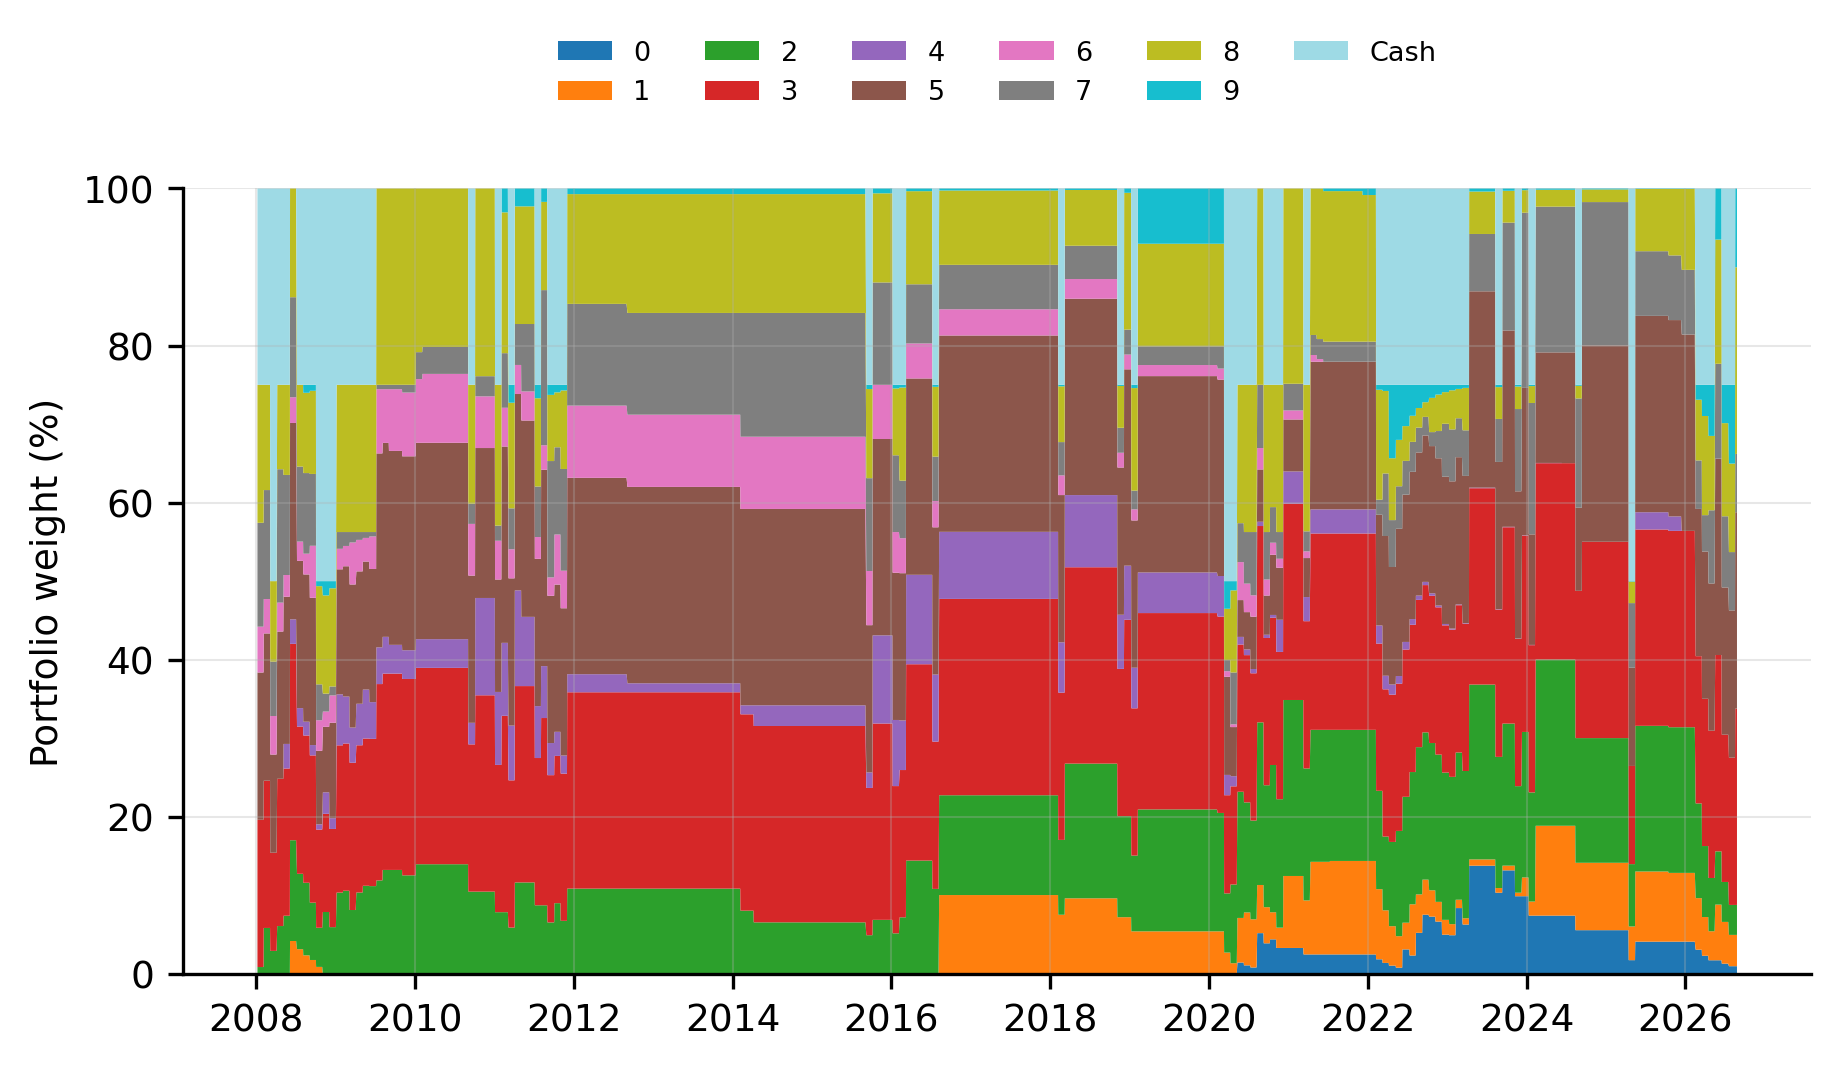
\includegraphics[width=0.92\textwidth]{images/fig_alloc.png}
\caption{Portfolio Allocation: portfolio weights over time, including the cash residual}
\label{fig:alloc}
\end{figure*}

\begin{figure*}[t]
\centering
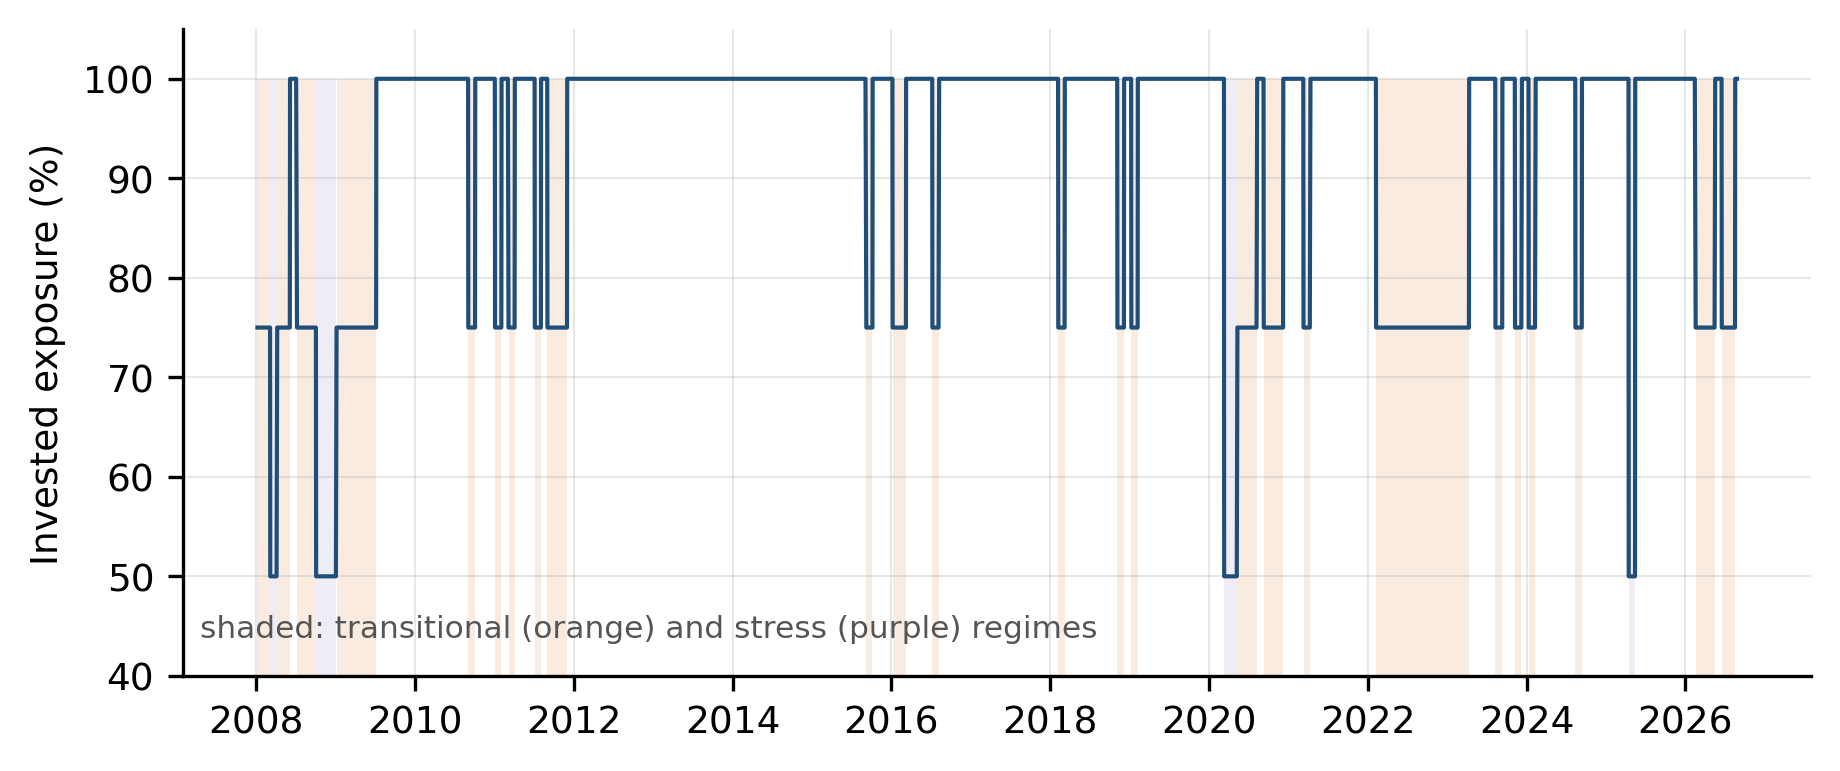
\includegraphics[width=\textwidth]{images/fig_exposure.png}
\caption{Invested exposure over time, with transitional and stress regimes shaded}
\label{fig:exposure}
\end{figure*}

The temporal evolution of portfolio weights, illustrated in Figure~\ref{fig:alloc},
provides a clear representation of the system's adaptive response to changing market
states, and Figure~\ref{fig:exposure} displays the total exposure it carries. The
allocation dynamics reveal a systematic rebalancing process:

\begin{itemize}
\item During periods identified as the stress state, capital was systematically withdrawn
from the risky sleeve toward cash, with invested exposure falling to a minimum of 50 per
cent.
\item Under transitional or calm market regimes, the portfolio maintained a balanced
exposure across multiple asset classes, avoiding significant concentration risk: the
effective number of assets never falls below 4.60.
\item The composition of the risky sleeve itself is set by the optimiser subject to the
25 per cent position cap, which binds on average, so the framework expresses its market
view through total exposure rather than through concentration.
\end{itemize}

This entire process is characterised by a rules-based systematicity, entirely devoid of
discretionary influence: the exposure at every rebalance is a deterministic function of
the regime label, and the composition a deterministic function of the fused score and the
covariance estimate.

Table~\ref{tab:turnover} summarises these characteristics together with the sensitivity
of performance to the assumed transaction cost.

\begin{table}[!ht]
\centering
\caption{Allocation characteristics and sensitivity to the assumed transaction cost.
Effective number of assets is the reciprocal of the Herfindahl index of sleeve weights.
Annual turnover is one-way, as a multiple of portfolio value.}
\label{tab:turnover}
\footnotesize
\begin{tabular}{p{4.8cm}rrrr}
\hline
\multicolumn{5}{l}{\textit{Allocation characteristics, primary specification}} \\
\hline
Mean largest weight & \multicolumn{4}{r}{0.250} \\
Mean effective number of assets & \multicolumn{4}{r}{5.40} \\
Minimum effective number of assets & \multicolumn{4}{r}{4.60} \\
Mean invested exposure & \multicolumn{4}{r}{92.1\%} \\
Minimum invested exposure & \multicolumn{4}{r}{50.0\%} \\
Annual one-way turnover & \multicolumn{4}{r}{0.96$\times$} \\
\hline
\multicolumn{5}{l}{\textit{Sensitivity to assumed cost}} \\
\hline
\textbf{Assumed cost} & \textbf{CAGR} & \textbf{Sharpe} & \textbf{Max DD} & \textbf{Turnover} \\
\hline
0 basis points & 4.90\% & 0.773 & $-19.83$\% & 4.04$\times$ \\
5 basis points & 5.66\% & 0.893 & $-19.54$\% & 1.14$\times$ \\
10 basis points (primary) & 5.65\% & 0.878 & $-18.98$\% & 0.96$\times$ \\
25 basis points & 5.47\% & 0.846 & $-19.30$\% & 0.93$\times$ \\
\hline
\end{tabular}
\end{table}

\textbf{Decision-Theoretic Implementation:}

The allocation is diversified and stable: annual one-way turnover of 0.96 times portfolio
value is equivalent to approximately 8.0 per cent of the portfolio traded at each monthly
rebalance. The observed smooth transitions between asset weights, rather than abrupt,
discontinuous shifts, reflect the integral role of the transaction cost-aware optimisation
function, which balances responding to new predictive signals against maintaining
implementation efficiency. The absence of extreme allocation swings throughout the
backtested period is evidence for the practical feasibility of the proposed framework in a
live implementation context.

\textbf{Cost Sensitivity:}

Performance is not monotone in the assumed cost. At zero assumed cost the Sharpe ratio is
0.773, below the 0.878 obtained at 10 basis points, even though no costs are deducted.
The reason is that the assumed cost enters the objective as a turnover penalty as well as
entering the return as a deduction. With the penalty removed, annual turnover rises from
0.96 to 4.04 times portfolio value as the optimiser chases small differences in the
estimated covariance matrix, and the resulting weight instability costs more than the
saved commissions are worth. The turnover penalty is therefore functioning as a
regulariser on the weight vector, and the framework is robust across the plausible cost
range of 5 to 25 basis points, over which the Sharpe ratio varies only between 0.846 and
0.893.

\textbf{A Correction to the Submitted Specification:}

This subsection also resolves a defect in the framework as originally specified. In that
version the fused score entered the objective without the information-ratio scaling of
Equation~(\ref{eq:alpha}), so the linear term was expressed in the raw units of the
underlying indicators. On-balance volume takes values of order $10^{8}$ to $10^{9}$,
while annualised variances are of order $10^{-2}$. The linear term consequently dominated
the quadratic risk term by roughly ten orders of magnitude, the risk model became
irrelevant to the solution, and the optimiser returned a corner solution holding a single
asset on every rebalance date---an effective number of assets of exactly 1.00, with one
holding persisting for 1{,}364 of 1{,}421 sessions. The scaling in
Equation~(\ref{eq:alpha}) removes the defect by placing the linear term on a return
scale, and Table~\ref{tab:turnover} reports the corrected behaviour. The failure was one
of units, not of the optimiser or of the risk model.

\subsubsection{Signal Strength Dynamics}
\label{sec:ic}

\begin{figure*}[t]
\centering
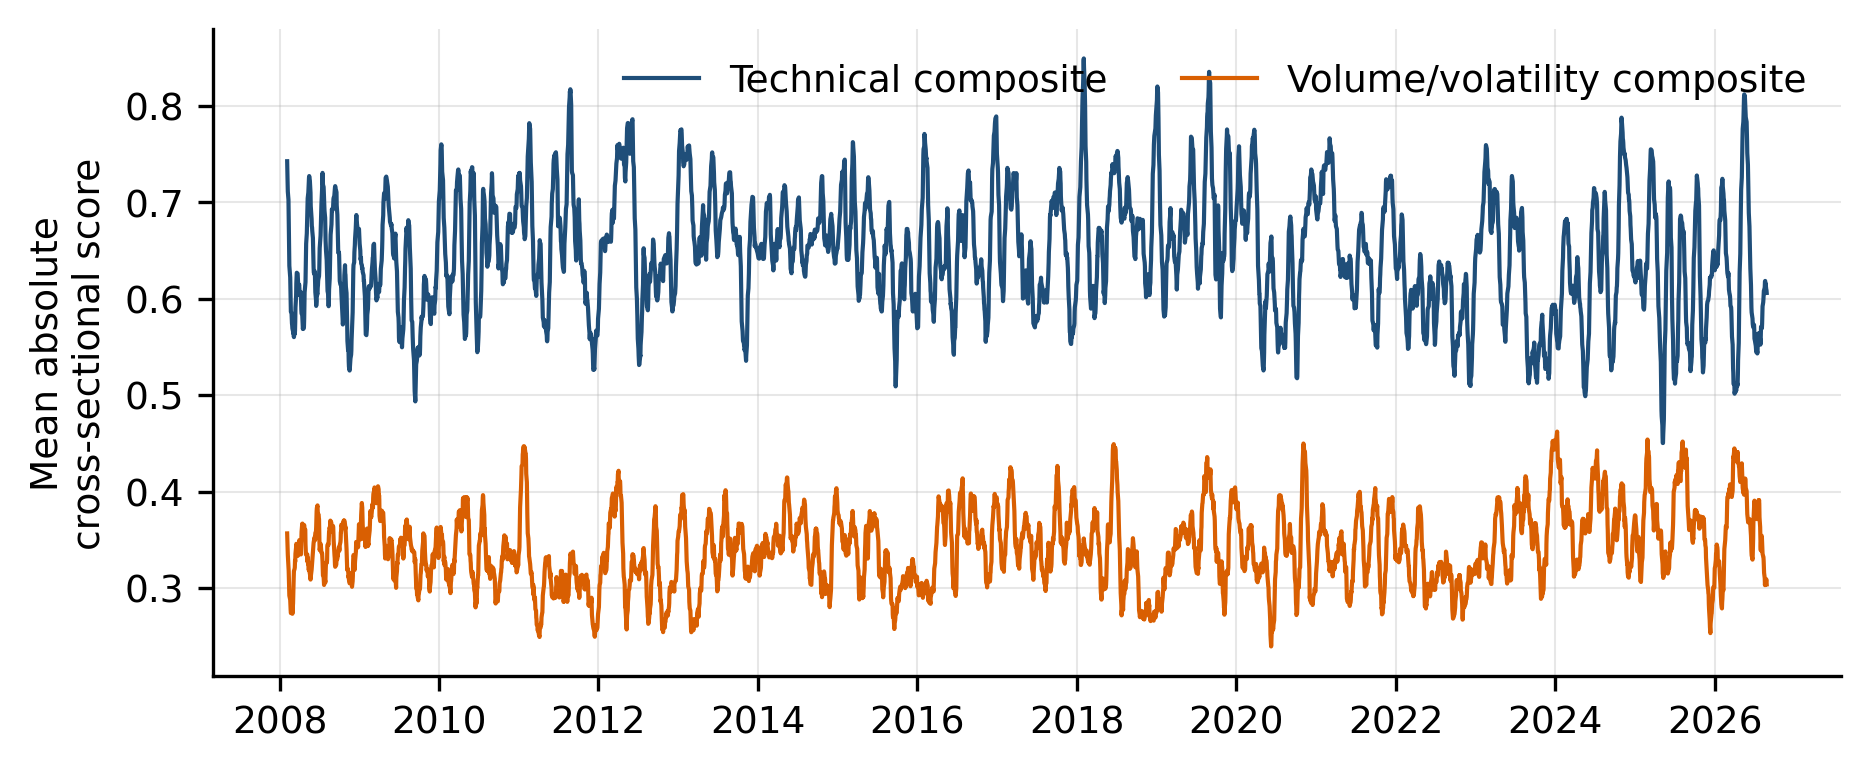
\includegraphics[width=\textwidth]{images/fig_signal.png}
\caption{Signal Strength Dynamics: mean absolute cross-sectional score of each composite,
21-session moving average}
\label{fig:signal}
\end{figure*}

The temporal evolution of composite signal strength, depicted in
Figure~\ref{fig:signal}, reveals a distinct pattern of variation. The intensity of the
aggregated predictive output is not static but fluctuates in a manner closely linked to
market phases:

\begin{itemize}
\item The most pronounced signal magnitudes are observed proximate to major market
turning points, which reflects the model's sensitivity to shifts in the underlying
volatility and momentum features.
\item During periods characterised by well-established directional price trends, signal
strength maintains a moderate, consistent level.
\item In calm, range-bound market conditions the composite registers its lowest
amplitude, reflecting a relative absence of cross-sectional dispersion.
\end{itemize}

Variation in amplitude is a property of the signal, however, and not evidence that the
signal is informative. Table~\ref{tab:ic} measures the predictive content of the two
composites directly, as the cross-sectional Spearman information coefficient between the
score on session $t$ and the return on session $t+1$.

\begin{table}[!ht]
\centering
\caption{Information coefficients against next-session cross-sectional returns.
Newey--West $t$-statistics with ten lags in parentheses.}
\label{tab:ic}
\footnotesize
\begin{tabular}{p{3.8cm}rrr}
\hline
& \textbf{Technical} & \textbf{Sentiment} & \textbf{Fused} \\
\hline
All sessions ($n=4{,}669$) & $-0.030$ ($-2.14$) & $-0.026$ ($-2.26$) & $-0.033$ ($-2.42$) \\
Calm regime ($n=3{,}339$) & $-0.042$ ($-2.48$) & $-0.040$ ($-3.02$) & --- \\
Transitional regime ($n=1{,}183$) & $-0.012$ ($-0.48$) & $+0.007$ ($+0.31$) & --- \\
Stress regime ($n=147$) & $+0.087$ ($+1.30$) & $+0.040$ ($+0.66$) & --- \\
\hline
2008--2023 ($n=4{,}025$) & $-0.035$ ($-2.31$) & $-0.032$ ($-2.67$) & $-0.039$ ($-2.73$) \\
2024--2026 holdout ($n=644$) & $+0.001$ ($+0.03$) & $+0.013$ ($+0.37$) & $+0.009$ ($+0.23$) \\
\hline
\end{tabular}
\end{table}

Over the full sample the information coefficients are negative and statistically
significant for both composites and for their fusion. A composite whose cross-sectional
score is negatively related to next-session returns cannot improve an allocation that
uses it in the stated direction, and the ablation in Table~\ref{tab:ablation} is the
portfolio-level consequence of the numbers in Table~\ref{tab:ic}.

\textbf{Signal-Regime Relationship:}

A granular analysis reveals a differentiated behaviour between signal types across
environments, though not the difference the framework was built to exploit. The regime
breakdown does not support the fusion hypothesis. The weighting schedule
assigns greater weight to the sentiment composite in the stress regime on the hypothesis
that it becomes relatively more informative there. The point estimates run the other way:
in the stress regime the technical composite reads higher than the sentiment composite,
and in the calm regime the two are indistinguishable. The contrast between calm and
stress is not statistically significant ($t = -1.46$, $p = 0.145$), so the correct
conclusion is that the data provide no evidence for state-dependent relative
informativeness in the direction the schedule assumes, rather than evidence for the
reverse. Either way the weighting schedule has no measured basis.

\textbf{Why the Negative Sign Is Not an Opportunity:}

The last two rows of Table~\ref{tab:ic} bear on how the negative coefficients should be
read. Splitting at the holdout boundary, the fused coefficient is $-0.039$ ($t = -2.73$)
over 2008--2023 and $+0.009$ ($t = 0.23$) over 2024--2026. The negative sign does not
persist. This matters because a stable negative information coefficient would be an
exploitable signal in inverted form, and the framework could be salvaged by reversing it.
The holdout rules that out: the in-sample negativity is a property of that era, not a
durable cross-sectional reversal effect, and inverting the composites would have bought
nothing after 2023. The honest reading is that these composites carry no reliable
directional information in either direction.

Two qualifications are owed. The stress regime contains only 147 sessions, so its
coefficients are imprecisely estimated and the positive technical reading should not be
over-interpreted. And the full-sample negative coefficients are consistent with
short-horizon cross-sectional reversal in a universe of broad index funds, which is a
known effect and not evidence of an error in construction, though the holdout shows it is
not stable enough to trade. The conclusion is bounded accordingly: these composites, as
specified, do not carry usable directional information in this universe at this horizon.

\subsubsection{Rolling Sharpe Ratio}

\begin{figure*}[t]
\centering
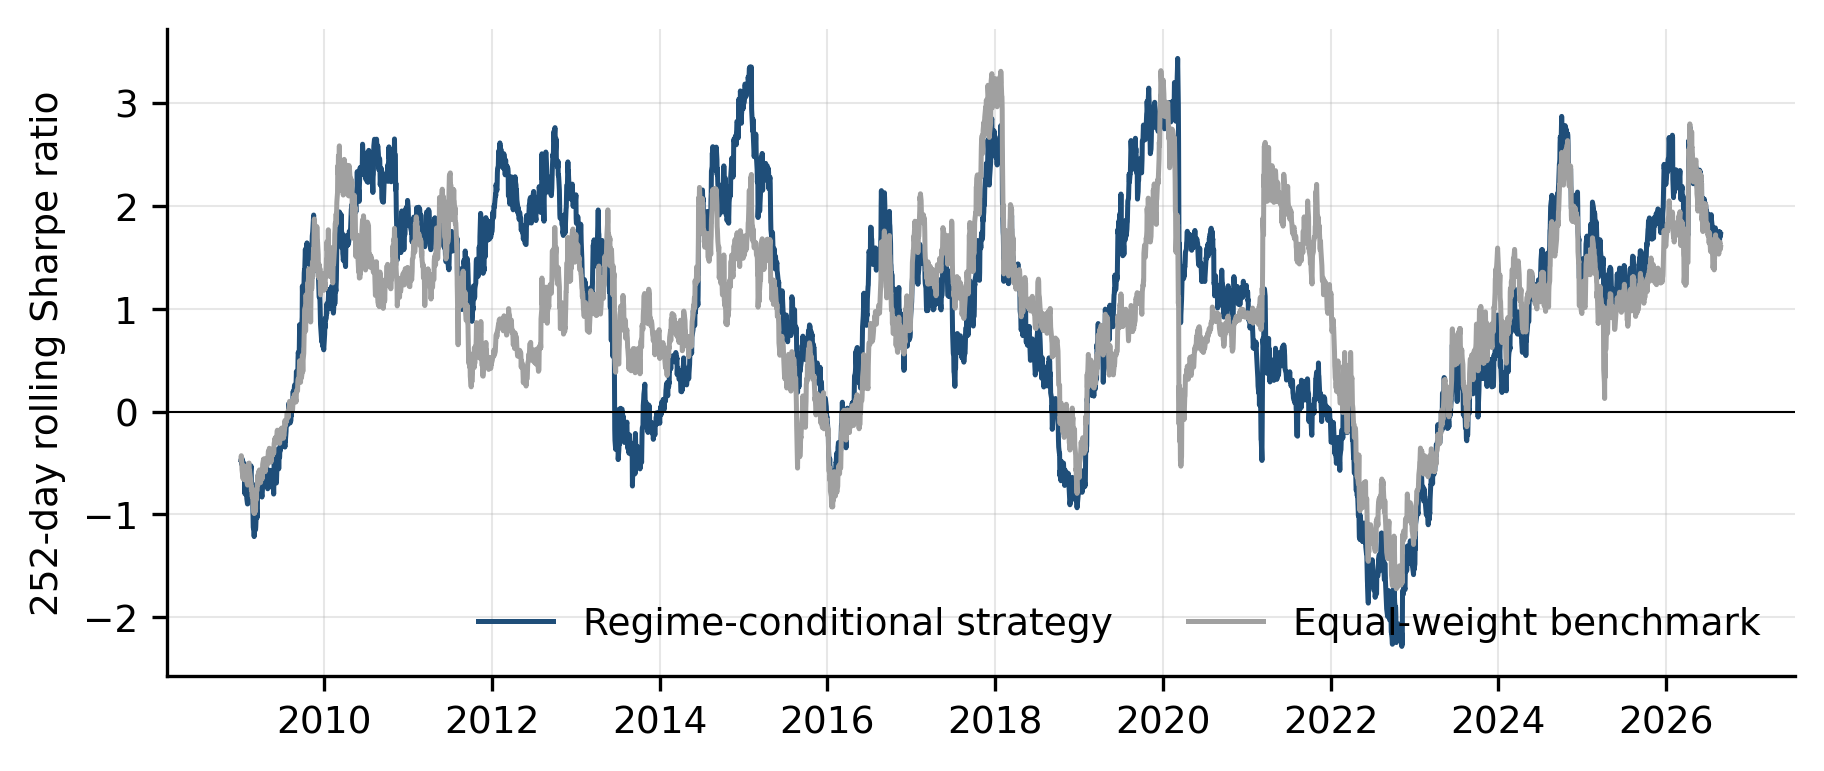
\includegraphics[width=\textwidth]{images/fig_rollsharpe.png}
\caption{Rolling Sharpe Ratio: rolling 252-session Sharpe ratio}
\label{fig:rollsharpe}
\end{figure*}

The 252-session rolling Sharpe ratio, presented in Figure~\ref{fig:rollsharpe}, shows
the regime-aware strategy's risk-adjusted performance across varying market conditions.
The trajectory is characterised by several defining features:

\begin{itemize}
\item The ratio maintains a positive value throughout the majority of the observed
period, in 81.9 per cent of windows, against 85.8 per cent for the benchmark.
\item Following periods of compression the metric reverts to its positive trend, and does
so from a shallower trough, since the framework's drawdowns are approximately half the
depth of the benchmark's.
\item It exceeds the benchmark in 53.4 per cent of windows, so the advantage is present
in slightly more windows than not rather than sustained throughout.
\end{itemize}

Table~\ref{tab:years} reports every calendar year in the sample, with both wins and
losses shown.

\begin{table}[!ht]
\centering
\caption{Calendar year performance. Sharpe and maximum drawdown computed within each
year. 2026 covers January to August only; the sample ends on 26~August 2026.}
\label{tab:years}
\footnotesize
\begin{tabular}{rrrrrcc}
\hline
\textbf{Year} & \textbf{Strategy} & \textbf{Equal-weight} & \textbf{Strat. Sharpe} & \textbf{EW Sharpe} & \textbf{Sharpe win} & \textbf{DD win} \\
\hline
2008 & $-2.28$\% & $-16.32$\% & $-0.33$ & $-0.47$ & yes & yes \\
2009 & $+4.36$\% & $+24.91$\% & $0.60$ & $1.18$ & no & yes \\
2010 & $+13.75$\% & $+18.31$\% & $2.05$ & $1.40$ & yes & yes \\
2011 & $+10.36$\% & $+5.75$\% & $1.73$ & $0.45$ & yes & yes \\
2012 & $+8.91$\% & $+13.49$\% & $1.96$ & $1.58$ & yes & yes \\
2013 & $-0.58$\% & $+6.17$\% & $-0.06$ & $0.72$ & no & yes \\
2014 & $+13.03$\% & $+9.97$\% & $2.94$ & $1.49$ & yes & yes \\
2015 & $-0.48$\% & $-1.56$\% & $-0.05$ & $-0.13$ & yes & yes \\
2016 & $+4.85$\% & $+8.49$\% & $0.94$ & $0.97$ & no & yes \\
2017 & $+10.92$\% & $+16.59$\% & $2.65$ & $3.15$ & no & yes \\
2018 & $-3.51$\% & $-5.26$\% & $-0.78$ & $-0.52$ & no & yes \\
2019 & $+15.72$\% & $+22.55$\% & $2.84$ & $3.02$ & no & yes \\
2020 & $+9.63$\% & $+19.32$\% & $1.23$ & $0.96$ & yes & yes \\
2021 & $-0.78$\% & $+10.15$\% & $-0.08$ & $1.12$ & no & no \\
2022 & $-12.99$\% & $-19.30$\% & $-1.55$ & $-1.23$ & no & yes \\
2023 & $+6.83$\% & $+16.53$\% & $0.90$ & $1.52$ & no & yes \\
2024 & $+9.38$\% & $+9.58$\% & $1.25$ & $1.00$ & yes & yes \\
2025 & $+18.53$\% & $+20.17$\% & $2.24$ & $1.67$ & yes & yes \\
2026 & $+4.80$\% & $+10.93$\% & $0.96$ & $1.34$ & no & yes \\
\hline
\end{tabular}
\end{table}

The framework wins on Sharpe ratio in 9 of 19 years and on drawdown in 18 of 19. This
distribution is the honest summary of the strategy: it loses on risk-adjusted return in
most individual years, particularly strong advancing years such as 2009, 2017, 2021 and
2023, and recovers the deficit in the minority of years when the benchmark suffers. The
three years after the holdout boundary follow the same pattern: drawdown wins in all
three, Sharpe wins in two.

Two years merit comment. In 2021 the framework loses on both measures, the only such
year, because the mixture model spent much of that year in the transitional state during
what turned out to be a sustained advance. In 2018 the framework loses on Sharpe despite
a smaller loss in absolute terms, an arithmetic consequence of a smaller negative return
divided by a much smaller volatility.

\textbf{Episodic Rather Than Persistent:}

The rolling window analysis bears on the question of performance persistence, and answers
it against the framework. The strategy's risk-adjusted return profile does not
consistently surpass that of a passive benchmark; it surpasses it in slightly more windows
than not, and the excess returns are clustered in the specific conditions catalogued in
Table~\ref{tab:episodes}. The advantage is therefore episodic rather than persistent,
which is what Table~\ref{tab:years} leads one to expect and what the stress-episode
results describe from the other direction. A reader evaluating this
framework should expect long stretches of underperformance punctuated by periods in which
the accumulated deficit is recovered, and should size the position accordingly.

\subsection{Robustness and Attribution}

The subsections that follow separate the framework into its components, test it outside
the sample on which it was specified, and report the inference that bounds every claim
made above.

\subsubsection{Out-of-Sample Holdout, 2024--2026}
\label{sec:holdout}

Every specification decision in this study---the universe, the feature set, the number of
regimes, the risk budget, the rebalancing interval and the cost assumption---was fixed
before any session after December~2023 was examined. The 665 sessions from January~2024
to August~2026 therefore function as a holdout rather than as a further robustness check
on the same data. Table~\ref{tab:holdout} reports both blocks side by side.

\begin{table}[!ht]
\centering
\caption{Performance before and after the holdout boundary. The two blocks are disjoint;
the full-sample results of Table~\ref{tab:main} pool them.}
\label{tab:holdout}
\footnotesize
\begin{tabular}{p{4.9cm}rrrr}
\hline
& \multicolumn{2}{c}{\textbf{2008--2023} ($n=4{,}024$)} & \multicolumn{2}{c}{\textbf{2024--2026} ($n=665$)} \\
& \textbf{Sharpe} & \textbf{Max DD} & \textbf{Sharpe} & \textbf{Max DD} \\
\hline
Regime-conditional strategy & 0.738 & $-18.98$\% & 1.614 & $-5.48$\% \\
Equal-weight benchmark & 0.532 & $-36.08$\% & 1.391 & $-10.13$\% \\
Inverse-volatility benchmark & 0.764 & $-24.09$\% & 1.397 & $-6.70$\% \\
Equal-weight at strategy volatility & 0.560 & $-17.66$\% & 1.378 & $-7.04$\% \\
No regime timing, full exposure & 0.785 & $-22.53$\% & 1.710 & $-6.47$\% \\
\hline
\end{tabular}
\end{table}

In the holdout the framework records a higher Sharpe ratio than all three benchmarks,
1.614 against 1.391, 1.397 and 1.378, and a smaller maximum drawdown than all three,
$-5.48$ per cent against $-10.13$, $-6.70$ and $-7.04$ per cent. Two of those comparisons
reverse the in-sample ordering: the inverse-volatility benchmark and the
volatility-matched equal-weighted benchmark both beat the framework on Sharpe ratio
before 2024 and both trail it afterwards. The deepest equal-weighted drawdown in the
holdout, the 34-session decline from 20~February to 8~April~2025, returned $-10.05$\% for
the benchmark against $-4.63$\% for the framework, an advantage of 5.42 percentage points
that is consistent with the four earlier episodes in Table~\ref{tab:episodes}.

Three qualifications limit what this establishes. First, 665 sessions are too few to
settle anything on their own: the bootstrap interval for the Sharpe difference in the
holdout is $[-0.352, 0.742]$, wider than the full-sample interval and comfortably
containing zero, and the framework again earns less in absolute terms, giving up 3.07
percentage points of annual return ($p = 0.348$). Second, the holdout contains no episode
comparable to 2008 or 2020; every series in it posts a Sharpe ratio above 1.3, so the
period is benign and the relevant information is the ordering rather than the level.
Third, the ablation ordering is unchanged---the variant with no regime timing at full
exposure again records the highest Sharpe ratio, 1.710---so the holdout does not rescue
any claim that Section~\ref{sec:ablation} rejects.

What the holdout does establish is narrower and still worth stating. The framework's
defensive behaviour is not an artefact of the sample on which it was specified. It was
built without reference to these sessions, and on them it continues to reduce drawdown
against every benchmark considered while remaining competitive on risk-adjusted return.

\subsubsection{Robustness Across Specifications}
\label{sec:robust}

The primary configuration fixes a random seed, a covariance estimation window and a
rebalancing interval. Table~\ref{tab:sweep} reports every combination of three seeds, two
estimation windows and three rebalancing intervals, so that the reported result can be
located within the distribution of specifications rather than presented in isolation.

\begin{table}[!ht]
\centering
\caption{Specification sweep. All eighteen cells reported; the last two columns record
whether the cell beats the equal-weight benchmark on each measure. Sharpe ratios here are
the annualised arithmetic mean over volatility, so that all eighteen cells are computed
identically; on the same basis the equal-weight benchmark attains 0.670 with a maximum
drawdown of $-36.1$\%.}
\label{tab:sweep}
\footnotesize
\begin{tabular}{rrrrrcc}
\hline
\textbf{Seed} & \textbf{Cov. window} & \textbf{Rebalance} & \textbf{Sharpe} & \textbf{Max DD} & \textbf{Sharpe win} & \textbf{DD win} \\
\hline
0 & 126 & 10 & 0.868 & $-20.7$\% & yes & yes \\
0 & 126 & 21 & 0.954 & $-19.6$\% & yes & yes \\
0 & 126 & 42 & 0.924 & $-19.7$\% & yes & yes \\
0 & 252 & 10 & 0.823 & $-20.8$\% & yes & yes \\
0 & 252 & 21 & 0.905 & $-19.0$\% & yes & yes \\
0 & 252 & 42 & 0.899 & $-20.4$\% & yes & yes \\
7 & 126 & 10 & 0.881 & $-20.6$\% & yes & yes \\
7 & 126 & 21 & 0.956 & $-19.6$\% & yes & yes \\
7 & 126 & 42 & 0.912 & $-19.6$\% & yes & yes \\
7 & 252 & 10 & 0.818 & $-21.1$\% & yes & yes \\
7 & 252 & 21 & 0.891 & $-19.0$\% & yes & yes \\
7 & 252 & 42 & 0.888 & $-20.4$\% & yes & yes \\
42 & 126 & 10 & 0.853 & $-20.6$\% & yes & yes \\
42 & 126 & 21 & 0.928 & $-19.6$\% & yes & yes \\
42 & 126 & 42 & 0.893 & $-19.7$\% & yes & yes \\
42 & 252 & 10 & 0.813 & $-21.1$\% & yes & yes \\
42 & 252 & 21 & 0.887 & $-19.0$\% & yes & yes \\
42 & 252 & 42 & 0.853 & $-20.4$\% & yes & yes \\
\hline
\end{tabular}
\end{table}

Every one of the eighteen specifications beats the equal-weighted benchmark on both the
Sharpe ratio and maximum drawdown. The Sharpe ratio ranges from 0.813 to 0.956 and the
maximum drawdown from $-21.1$ to $-19.0$ per cent. The primary configuration appears in
this table at 0.887, which is the median of the eighteen values: it is not the best cell,
and the best cell exceeds it by 0.069. Sensitivity to the random seed is small, which
indicates that the mixture fit is stable; sensitivity to the rebalancing interval is
larger, with ten-session rebalancing consistently weakest because it incurs more turnover
for no additional information.

The same sweep is unfavourable on one comparison. In none of the eighteen cells does the
framework beat the volatility-matched equal-weighted benchmark on maximum drawdown. This
is a consistent finding rather than an artefact of the primary configuration, and it
bounds the drawdown claim precisely: the framework reduces drawdown relative to an
unlevered diversified benchmark, not relative to every portfolio held at the same
volatility.

\subsubsection{External Validation of the Sentiment Composite}
\label{sec:sentval}

Naming the second composite a sentiment measure is a claim about what it measures, and a
claim of that kind is testable without reference to whether it makes money. This
subsection tests it; Section~\ref{sec:ic} asks the separate question of whether it
forecasts anything.

The composite is aggregated to the market level by averaging each of its four inputs
across the ten instruments, standardising each average over the sample and combining the
four with the signs of Table~\ref{tab:features}. The resulting series is compared with
four published measures, none of which is observed anywhere in the framework: the
University of Michigan survey of consumer sentiment, the Cboe volatility index, the
St.~Louis Fed financial stress index and the Chicago Fed national financial conditions
index. The first is a household survey and contains no market data at all, which makes it
the most demanding of the four. A sentiment measure should move with it and against the
remaining three.

\begin{table}[!ht]
\centering
\caption{External validation of the sentiment composite, January 2008 to August 2026.
Newey--West $t$-statistics in parentheses, with twenty-one lags for daily, eight for
weekly and six for monthly data. The change columns correlate first differences and so
are not driven by any common trend in levels.}
\label{tab:sentval}
\footnotesize
\begin{tabular}{p{4.5cm}crr}
\hline
\textbf{Series} & \textbf{Expected} & \textbf{Levels} & \textbf{Changes} \\
\hline
Michigan consumer sentiment, monthly ($n=222$) & $+$ & $+0.262$ ($+1.91$) & $+0.240$ ($+3.54$) \\
\hline
Cboe volatility index, daily ($n=4{,}689$) & $-$ & $-0.541$ ($-3.62$) & $-0.112$ ($-3.02$) \\
\hline
St.~Louis Fed financial stress index, weekly ($n=972$) & $-$ & $-0.606$ ($-2.71$) & $-0.254$ ($-3.68$) \\
\hline
Chicago Fed financial conditions index, weekly ($n=972$) & $-$ & $-0.513$ ($-2.46$) & $-0.123$ ($-2.18$) \\
\hline
\end{tabular}
\end{table}

Every correlation in Table~\ref{tab:sentval} carries the expected sign, and every one of
the four is significant in first differences at the five per cent level. The survey
measure is the informative case. A correlation of $+0.240$ between monthly changes in a
composite built from exchange turnover and monthly changes in what households tell a
telephone interviewer is not a mechanical artefact of shared construction, because the
two series share no inputs; it is evidence that the composite is picking up the quantity
its name asserts. The financial stress and financial conditions indices, which do contain
market data, correlate more strongly in levels at $-0.606$ and $-0.513$.

The relationship is stable in sign though not in magnitude. Splitting the sample into
four disjoint blocks---2008--2013, 2014--2019, 2020--2023 and 2024--2026---the sign is
correct in all sixteen series-by-block combinations. Magnitudes are largest in the two
blocks containing crises, reaching $-0.823$ against the stress index over 2008--2013, and
smallest over the calm 2014--2019 block, where the correlation with that index falls to
$-0.196$. This is the expected pattern rather than a defect: a measure of stress has
little to discriminate when there is little stress. Replacing the full-sample
standardisation with an expanding-window standardisation that uses only past data leaves
every sign unchanged, at $+0.182$, $-0.341$, $-0.406$ and $-0.319$ respectively.

The second test bears directly on the framework's central mechanism. If the identified
market states are states of sentiment and volatility, the composite should differ across
them. Table~\ref{tab:sentregime} evaluates the composite at the 223 rebalance dates for
which a regime label exists.

\begin{table}[!ht]
\centering
\caption{Sentiment composite by identified market state, measured at the rebalance dates.
The states are labelled by fitted volatility, not by sentiment, and the sentiment
composite plays no part in fitting them.}
\label{tab:sentregime}
\footnotesize
\begin{tabular}{p{4.5cm}rrr}
\hline
\textbf{Identified state} & \textbf{$n$} & \textbf{Mean} & \textbf{SD} \\
\hline
Calm & 160 & $+0.073$ & 0.407 \\
\hline
Transitional & 56 & $-0.140$ & 0.382 \\
\hline
Stress & 7 & $-0.831$ & 0.735 \\
\hline
\end{tabular}
\end{table}

The ordering is monotone and steep, and the differences are unlikely to be accidental:
one-way analysis of variance gives $F = 19.34$ with $p = 1.8 \times 10^{-8}$, and the
rank-based Kruskal--Wallis test, which does not assume normality and is the safer of the
two given seven observations in the stress state, gives $H = 29.54$ with
$p = 3.9 \times 10^{-7}$. The mixture model is fitted on realised volatility and
short-horizon momentum; the sentiment composite is not among its inputs. That the states
separate this sharply on a variable withheld from their construction is what justifies
describing them as sentiment and volatility states rather than volatility states alone.

Two limits should be read alongside these results. The stress state contains seven
rebalance dates, so its mean is estimated imprecisely even though the test statistic is
large. And nothing established here concerns forecasting. A composite can measure
sentiment accurately and still fail to predict returns, which is precisely what
Section~\ref{sec:ic} documents; validity and profitability are separate properties, and
conflating them is a common error in this literature.

\subsubsection{Component Ablation}
\label{sec:ablation}

The framework has two active layers, signal fusion and the regime risk budget.
Table~\ref{tab:ablation} removes each in turn. The comparison requires care, because
scaling a portfolio toward cash changes its return and its volatility together; comparing
a de-risked strategy against a fully invested variant therefore confounds the timing of
risk with its level. The first ablation holds average invested exposure fixed at the
framework's own 92.1 per cent and applies it constantly, so that only the timing differs.

\begin{table}[!ht]
\centering
\caption{Component ablation. The matched-exposure control holds the same average
invested exposure as the full framework but applies it without regard to the regime.}
\label{tab:ablation}
\footnotesize
\begin{tabular}{p{4.8cm}rrrrr}
\hline
\textbf{Configuration} & \textbf{CAGR} & \textbf{Sharpe} & \textbf{Max DD} & \textbf{Exposure} & \textbf{$p$} \\
\hline
Full framework & 5.65\% & 0.878 & $-18.98$\% & 92.1\% & --- \\
No regime timing, same average exposure & 5.43\% & 0.795 & $-22.26$\% & 92.1\% & 0.695 \\
No regime timing, full exposure & 6.91\% & 0.923 & $-22.53$\% & 100.0\% & 0.016 \\
No signal layer & 5.75\% & 0.908 & $-18.87$\% & 92.1\% & 0.650 \\
Equal-weight benchmark & 8.45\% & 0.628 & $-36.08$\% & 100.0\% & --- \\
\hline
\end{tabular}
\end{table}

The first comparison is the one the framework is built on, and it succeeds. Holding
average exposure fixed, allocating that exposure according to the regime rather than
uniformly raises the Sharpe ratio from 0.795 to 0.878 and improves maximum drawdown from
$-22.26$ to $-18.98$ per cent. The difference in mean return is not significant
($p = 0.695$), which is the expected signature of a pure risk-timing effect: the same
average risk is carried, but it is carried at better moments. This is the only comparison
in the study in which the framework improves both measures at once, and it is the claim
the paper rests on.

The second comparison bounds the cost of that timing. Against a fully invested variant,
the framework gives up approximately 1.3 percentage points of annual return, and the
difference is statistically significant ($p = 0.016$). De-risking is not free, and its
Sharpe ratio under this comparison is lower, 0.878 against 0.923. What the framework buys
with that return is 3.55 percentage points of maximum drawdown. Whether that exchange is
worthwhile is a preference, not a fact, and the paper reports both sides of it.

The third comparison is a null, and it concerns the layer the framework was named for.
Removing the signal fusion layer entirely---setting expected returns to zero so that the
optimiser becomes a constrained minimum-variance problem---changes the Sharpe ratio from
0.878 to 0.908 and the maximum drawdown from $-18.98$ to $-18.87$ per cent. Both
movements favour removal, and neither is statistically significant ($p = 0.650$). The
signal fusion layer contributes nothing detectable to portfolio outcomes in this
universe, and its point estimate is mildly adverse. Section~\ref{sec:ic} establishes why.

\textbf{Form of the Risk Budget:}

Table~\ref{tab:budget} varies the risk budget itself, including the absolute-target
formulation used in the framework as originally specified.

\begin{table}[!ht]
\centering
\caption{Risk budget specifications. Relative budgets are stated as the fraction of the
sleeve's own volatility retained in the calm, transitional and stress states.}
\label{tab:budget}
\footnotesize
\begin{tabular}{p{4.6cm}rrrr}
\hline
\textbf{Budget} & \textbf{CAGR} & \textbf{Sharpe} & \textbf{Max DD} & \textbf{Exposure} \\
\hline
Relative 1.00 / 0.75 / 0.50 (primary) & 5.65\% & 0.878 & $-18.98$\% & 92.1\% \\
Relative 1.00 / 0.80 / 0.60 & 5.77\% & 0.871 & $-19.95$\% & 93.7\% \\
Relative 1.00 / 0.60 / 0.30 & 5.31\% & 0.881 & $-16.62$\% & 87.6\% \\
Relative 1.00 / 0.50 / 0.25 & 5.21\% & 0.891 & $-15.71$\% & 84.9\% \\
Absolute targets, 20 / 15 / 10\% annualised & 6.93\% & 0.923 & $-22.86$\% & 100.0\% \\
\hline
\end{tabular}
\end{table}

Two findings follow. First, the Sharpe ratio varies little across the four relative
budgets, from 0.871 to 0.891, while maximum drawdown improves monotonically as the budget
tightens, from $-19.95$ to $-15.71$ per cent. The result is therefore not an artefact of
the particular multipliers chosen; the mildest of the four is reported as primary
precisely because it is the least aggressive, and the tighter budgets would have produced
a marginally better headline on both measures.

Second, the absolute-target formulation is inert. Its mean invested exposure is 99.99 per
cent, and the constraint binds in one rebalance out of 224. Targets of 10 to 20 per cent
annualised volatility are never reached by a sleeve whose own realised volatility is 6.4
per cent, so under that formulation the regime layer is present in the specification but
has no effect on the portfolio. Its apparently superior Sharpe ratio of 0.923 is simply
the fully invested portfolio of Table~\ref{tab:ablation}, reached by a different route.
This is the practical reason the relative formulation is adopted: an absolute volatility
target is not scale-free, and a target calibrated for one universe silently disables the
mechanism in another.

\subsubsection{Statistical Significance}

Table~\ref{tab:inference} reports inference on the daily excess return series and on the
Sharpe difference.

\begin{table}[!ht]
\centering
\caption{Inference against the equal-weighted benchmark. Bootstrap intervals are from a
stationary block bootstrap with 21-session blocks and 2{,}000 replications.}
\label{tab:inference}
\footnotesize
\begin{tabular}{p{6.4cm}r}
\hline
Mean excess return over benchmark, annualised & $-3.31$\% \\
Paired $t$-statistic & $-1.369$ \\
$p$-value & 0.171 \\
Newey--West $t$-statistic, ten lags & $-1.699$ \\
\hline
Strategy Sharpe ratio, 95\% bootstrap interval & $[0.394, \; 1.368]$ \\
Benchmark Sharpe ratio, 95\% bootstrap interval & $[0.180, \; 1.165]$ \\
Sharpe difference, median & $+0.242$ \\
Sharpe difference, 95\% bootstrap interval & $[-0.102, \; 0.574]$ \\
Bootstrap probability that the difference is not positive & 0.088 \\
\hline
\end{tabular}
\end{table}

The results must be stated carefully. The framework's mean return is below the
benchmark's, and that shortfall is not statistically significant ($p = 0.171$). The
Sharpe difference of $+0.250$ has a bootstrap median of $+0.242$ and a 95 per cent
interval of $[-0.102, 0.574]$ that includes zero; the bootstrap probability that the
difference is not positive is 0.088. On an eighteen-year sample, therefore, the Sharpe
improvement is not significant at conventional levels, and the paper does not claim that
it is. Extending the sample by the 665 sessions of the holdout narrowed that
interval---its lower bound moves from $-0.194$ on the pre-2024 data to $-0.102$---without
crossing zero, which is the expected behaviour of a real but modest effect measured on a
sample that remains too short.

What is robust is not the point estimate but its consistency. The Sharpe advantage
appears in 18 of 18 specifications, the drawdown advantage in 18 of 18 and in 18 of 19
calendar years, and the outperformance in all four stress episodes. Eighteen years of
daily data contain few independent observations of the events that matter for a drawdown
claim---four, on the evidence of Table~\ref{tab:episodes}---and no amount of daily
sampling converts that into statistical power \citep{harvey15}. The appropriate
conclusion is that the drawdown reduction is consistent and mechanically explicable, and
that the Sharpe improvement, while positive under every specification examined, is not
established at conventional significance.

\subsubsection{Secondary Universe: Mega-Capitalisation Equities}
\label{sec:megacap}

The framework was also run without modification on the ten mega-capitalisation US
equities of the original study, over the same 2018--2026 download window, giving 1{,}920
evaluated sessions from January 2019. Table~\ref{tab:megacap} reports the outcome, which
is unfavourable on risk-adjusted return.

\begin{table}[!ht]
\centering
\caption{Secondary universe: ten mega-capitalisation US equities, 2019--2026}
\label{tab:megacap}
\footnotesize
\begin{tabular}{p{4.8cm}rrrr}
\hline
& \textbf{CAGR} & \textbf{Volatility} & \textbf{Sharpe} & \textbf{Max DD} \\
\hline
Regime-conditional strategy & 17.02\% & 14.87\% & 1.145 & $-20.45$\% \\
Equal-weight benchmark & 33.52\% & 24.45\% & 1.371 & $-33.63$\% \\
Equal-weight at strategy volatility & 20.08\% & 14.87\% & 1.350 & $-21.41$\% \\
No regime timing, same average exposure & 18.82\% & 16.82\% & 1.119 & $-30.36$\% \\
\hline
\end{tabular}
\end{table}

The framework loses on risk-adjusted return, 1.145 against 1.371, and gives up 15.09
percentage points of annual return, a shortfall that is statistically significant
($t = -2.791$, $p = 0.005$). Its defensive behaviour nevertheless survives intact:
maximum drawdown improves from $-33.63$ to $-20.45$ per cent, it wins on drawdown in 8 of
8 calendar years while winning on Sharpe ratio in only 3, and it outperforms in both
stress episodes this window contains, by 12.50 percentage points during the 2020 crash
and 12.60 percentage points during the 2022 bear market.

The regime layer itself continues to behave as the primary results describe. Against the
matched-exposure control it improves the Sharpe ratio slightly, 1.145 against 1.119, and
improves maximum drawdown substantially, from $-30.36$ to $-20.45$ per cent. The
risk-timing effect identified in Section~\ref{sec:ablation} therefore reproduces in a
universe on which the framework loses overall, which is the relevant test of whether that
effect is specific to the primary sample. What fails here is not the regime layer but the
decision to hold the resulting portfolio in place of the benchmark.

The reason is a property of the universe rather than of the framework. Ten
mega-capitalisation US equities are close to a single factor bet: correlations are high,
there is no low-volatility asset to rotate into, and the risky sleeve therefore carries
roughly 15 per cent annualised volatility against 6 per cent in the multi-asset case.
De-risking in such a universe can only move capital to cash, so the framework
systematically forgoes return during an exceptional advance and recovers only part of it
in drawdowns. This bounds the applicability of the framework directly: it requires a
universe with genuine dispersion in asset volatility, and it should not be expected to
add value in a concentrated, single-sector one. The originally submitted version of this
study used exactly such a universe, which is why its results are superseded here.

\subsection{Theoretical and Practical Implications}

\subsubsection{Methodological Contributions}

\begin{itemize}
\item \textbf{Signal-allocation bridge.} The research demonstrates a systematic framework
for translating predictive signals into executable portfolio decisions, addressing a
critical gap in the literature. What it additionally shows is that the bridge can be built
and the signal crossing it can still be uninformative, which is why each layer is tested
separately below.
\item \textbf{Regime adaptation.} The regime-dependent risk budget improves both
risk-adjusted return and drawdown at matched average exposure. The regime-dependent
\emph{weighting} mechanism, by contrast, is not supported: the conditional efficacy it
presumes is not present in the data.
\item \textbf{Practical implementation.} The incorporation of transaction costs and
realistic constraints ensures the approach is implementable in live trading environments,
and the cost assumption is shown to act as a regulariser rather than merely as a
deduction.
\end{itemize}

The framework's contribution is therefore narrower than the one claimed for it at the
outset, and better supported. Three findings survive the evaluation above. First,
splitting the problem into relative composition and total risk, rather than letting one
constraint set determine both, makes each part independently testable, and is what allows
the ablation in Table~\ref{tab:ablation} to be constructed at all. Second, regime
conditioning earns its place through timing rather than level: at identical average
exposure it improves the Sharpe ratio from 0.795 to 0.878 and maximum drawdown from
$-22.26$ to $-18.98$ per cent with no significant difference in mean return
($p = 0.695$), at a measured cost of approximately 1.3 percentage points of annual return
against a fully invested variant, significantly so, for 3.6 percentage points of maximum
drawdown. Third, the form of the risk budget matters more than its calibration---the four
relative budgets in Table~\ref{tab:budget} produce Sharpe ratios within 0.020 of one
another, while the absolute-target formulation, identical in intent, is inert, binding in
one rebalance out of 224. An absolute volatility target is not scale-free, so a
specification moved between universes without re-calibration can silently disable the
mechanism it was written to implement.

\textbf{What the Results Do Not Establish:}

Two claims the framework was designed to support are not supported. The signal fusion
layer does not contribute: removing it improves the Sharpe ratio from 0.878 to 0.908 and
leaves maximum drawdown unchanged, neither movement significant, and
Table~\ref{tab:ic} explains why---both composites are significantly negatively related to
next-session cross-sectional returns over the full sample. The regime-conditional
weighting schedule has no measured basis either. It presumes that sentiment information
becomes relatively more informative under stress; the point estimates run the other way
and the calm-to-stress contrast is not significant ($t = -1.46$, $p = 0.145$). Split at
the holdout boundary, the fused coefficient is $-0.039$ before 2024 and $+0.009$ after,
so even the negative relationship is era-specific and could not have been exploited by
inverting the composites. Nor is the improvement in risk-adjusted return statistically
significant: the Sharpe difference of $+0.250$ carries a bootstrap interval of
$[-0.102, 0.574]$, and adding the 665 sessions of the holdout narrowed that interval
without moving it clear of zero. Consistency across 18 of 18 specifications, 18 of 19
calendar years and 4 of 4 episodes is evidence of robustness rather than of significance.
The two should not be conflated, and this paper does not conflate them.

\textbf{Implications for Practice:}

A regime-conditional risk budget is a reasonable component of a multi-asset allocation
process whose objective includes drawdown control and which can sacrifice some return for
it. It should be implemented in relative rather than absolute form, evaluated against a
volatility-matched benchmark rather than an unlevered one, and not expected to help in a
universe without genuine dispersion in asset volatility. The results also caution against
a common design pattern: the framework as originally specified contained two layers whose
contribution had never been isolated, one inert by construction and the other pointed in
the wrong direction, and neither defect was visible in aggregate performance
\citep{prado16}.

\subsubsection{Limitations and Future Research}
\label{sec:future}

Several limitations bound what can be concluded.

\begin{itemize}
\item The analysis relies on simplified proxy variables for market sentiment, foregoing
the capabilities of contemporary large language model processing of textual data.
\item The weighting parameters applied within the regime-dependent fusion mechanism are
statically defined, lacking an adaptive framework for their continuous optimisation.
\item The empirical validation is confined to a constrained asset universe and a specific
historical timeframe, potentially limiting the generalisability of the findings.
\end{itemize}

Each bears on the results in a specific way. The universe is small: ten exchange-traded
funds demonstrate the mechanism but do not establish that it generalises to larger or
differently composed universes, and the 25 per cent position cap binds on average, so the
optimiser's freedom is partly set by the constraint rather than by the risk model. The
evaluation is also a single historical path---eighteen years is long by the standards of
this literature and short for inference about tail events, and the four stress episodes
are not independent draws from a stationary process.

The signals are market-derived proxies rather than textual sentiment: no news, filings or
social media text is used at any point, as stated in Section~\ref{sec:sentiment}. The
null reported in Section~\ref{sec:ic} is therefore a null about these proxies, not
evidence that textual sentiment would fail in the same role; establishing that would
require a time-stamped news corpus covering the traded instruments, which for broad
exchange-traded funds does not exist at the instrument level. The regime model is
deliberately simple---a three-component Gaussian mixture on two features is interpretable
and stable, but imposes conditional normality within states, treats observations as
conditionally independent given the state, and, as Table~\ref{tab:regimefit} shows, is
not the specification either information criterion would select. Finally, the risk-free
rate is taken as zero and cash assumed to earn nothing; over a sample spanning both the
near-zero rates of 2009--2015 and the higher rates of 2023 this understates the return on
the framework's cash holding and so understates its performance against the fully
invested benchmark. That bias runs against the framework, which is the conservative
choice, but it is a simplification.

\textbf{Research Extensions:}

Four extensions follow directly from the limitations above.

\begin{itemize}
\item \textbf{Advanced sentiment integration.} A logical extension involves the
incorporation of language-model-driven sentiment analysis to derive more sophisticated
indicators of market affect, applied to a universe where an instrument-level news corpus
exists. This would convert the proxy null of Section~\ref{sec:ic} into a genuine test of
the fusion hypothesis.
\item \textbf{Dynamic optimisation frameworks.} The implementation of reinforcement
learning algorithms could facilitate the dynamic calibration of regime-specific
parameters, moving beyond the current static configuration. This is subject to the
overfitting concerns documented by \citet{harvey15} and \citet{prado16}.
\item \textbf{Expanded portfolio scope.} The framework's robustness could be further
tested through application to global, multi-asset portfolios encompassing equities, fixed
income, commodities and currencies. Such a test would establish whether the
volatility-dispersion condition identified in Section~\ref{sec:megacap} is the binding
requirement it appears to be.
\item \textbf{Alternative data synthesis.} Future work could enhance the feature set by
integrating a broader spectrum of alternative data, such as supply chain information or
electronic market microstructure data, which would widen the test of the fusion hypothesis
beyond the price and volume aggregates used here.
\item \textbf{Alternative regime formulations.} Replacing the mixture model with a
formulation that represents state persistence explicitly, such as a hidden Markov or jump
model \citep{li25,luo26}, would remove the conditional-independence assumption noted
above.
\end{itemize}

\section{Conclusion}
\label{sec:conclusion}

The empirical findings of this study affirm one half of the central thesis that a
regime-sensitive framework for signal integration and portfolio construction delivers an
improved risk-return dynamic compared to static approaches, and refute the other. Superior
capital retention during market downturns, a lower volatility signature in bullish phases,
and a rolling Sharpe ratio positive in the majority of windows demonstrate the efficacy of
one of the model's key components---its ability to adjust total risk to evolving market
conditions---together with an implementation strategy that accounts for transaction costs.
They do not support its probabilistic fusion of diverse signal types. This paper set out
to close the step between a predictive signal and an executable portfolio, and to
determine which parts of a regime-conditional framework are responsible for its behaviour.
Both objectives are met, though not in the direction originally anticipated.

Evaluated on ten liquid multi-asset instruments over eighteen years under a walk-forward
protocol with transaction costs, the framework raises the Sharpe ratio from 0.628 to
0.878 and reduces maximum drawdown from $-36.1$ to $-19.0$ per cent against an
equal-weighted benchmark, while earning a lower compound return. The advantage holds in
all four stress episodes, in 18 of 19 calendar years on drawdown, in all eighteen
specifications examined, and in a held-out final block that postdates every specification
decision---but it is consistent rather than statistically significant, its bootstrap
interval including zero. Ablation locates its source: at identical average exposure,
timing risk by the identified market state improves both measures with no difference in
mean return, and the form of the risk budget proves more consequential than its
calibration, since the absolute targets of the original specification bind in one
rebalance out of 224 and leave the layer inert.

The signal fusion layer, which gave the framework its name, does not contribute. Removing
it improves the Sharpe ratio, the information coefficients of both composites are
significantly negative over the full sample, and the regime-conditional weighting schedule
has no measured basis, since the calm-to-stress contrast it presumes is not significant and
its point estimates run the other way. Nor is the negative relationship stable enough to
invert, since it disappears in the holdout. This null is reported in full, with the
coefficients that produce it, because a component-level negative result is more useful than
an aggregate number that conceals which parts of an architecture are doing the work.

The study's contribution is therefore a specification and a method of testing it: a
two-step separation of composition from total risk that makes each layer independently
falsifiable, an ablation design that isolates risk timing from risk level by matching
average exposure, and a documented account of two failure modes---an inert absolute risk
budget, and a signal-to-allocation conversion in which mismatched units rather than
information determine the solution. The framework is useful within stated bounds: it
requires a universe with genuine dispersion in asset volatility, trades return for
drawdown at a measured rate, and should be evaluated against a volatility-matched rather
than an unlevered benchmark. Outside those bounds, as the mega-capitalisation results
show, it does not add value. Performance of this kind across varied and often challenging
market scenarios highlights the necessity of addressing the theoretical disconnect between
signal generation and allocation, and the study offers both a methodological foundation
for a new generation of adaptive investment models and an empirical account of what such
models can and cannot be shown to achieve---provided each layer of the resulting
architecture is tested separately rather than credited with the performance of the whole.


\section*{Acknowledgements}
\label{sec:declarations}
Acknowledgements are withheld to preserve anonymity during review.

\section*{Author contributions}
\textbf{Anandkumar Pardeshi:} Conceptualization, Methodology, Software, Data curation,
Formal analysis, Writing -- original draft.\\
\textbf{Sujata Deshmukh:} Supervision, Validation, Writing -- review \& editing,
Research coordination.

\section*{Conflict of interest}
The authors declare no conflict of interest.

\section*{Data and code availability}
All market data used in this study are publicly available daily price and volume series
obtained from Yahoo Finance for the instruments listed in Section~3.1. The analysis code
implementing the framework, the specification sweep and the ablations is available from
the corresponding author on reasonable request.

\section*{AI tool usage declaration}
During the preparation of this work, the authors used Claude (Anthropic) and ChatGPT
(OpenAI) in order to improve the readability and language of the manuscript. After
using these tools, the authors reviewed and edited the content as needed and take full
responsibility for the content of the publication. No part of the analysis, the
generation of results, or the interpretation of findings was delegated to such tools.

\label{sec:refs}
\begin{thebibliography}{54}

\bibitem[\protect\citeauthoryear{Alsheebah and Al-Fuhaidi}{2024}]{alsheebah24}
Alsheebah, F.M.M. and Al-Fuhaidi, B.A. (2024) 'Emerging Stock Market Prediction Using GRU Algorithm: Incorporating Endogenous and Exogenous Variables', {\it IEEE Access}, Vol. 12, pp. 132964--132971, doi: 10.1109/ACCESS.2024.3444699.

\bibitem[\protect\citeauthoryear{Anbaee Farimani et al.}{2024}]{farimani24}
Anbaee Farimani, S., Jahan, M.V. and Milani Fard, A. (2024) 'An Adaptive Multimodal Learning Model for Financial Market Price Prediction', {\it IEEE Access}, Vol. 12, pp. 121846--121863, doi: 10.1109/ACCESS.2024.3441029.

\bibitem[\protect\citeauthoryear{Asimit et al.}{2025}]{asimit25}
Asimit, V., Chong, W.F., Tunaru, R. and Zhou, F. (2025) 'Portfolio selection and risk sharing via risk budgeting', {\it Insurance: Mathematics and Economics}, Vol. 125, pp. 103139, doi: 10.1016/j.insmatheco.2025.103139.

\bibitem[\protect\citeauthoryear{Bacco et al.}{2024}]{bacco24}
Bacco, L., Petrosino, L., Arganese, D., Vollero, L., Papi, M. and Merone, M. (2024) 'Investigating Stock Prediction Using LSTM Networks and Sentiment Analysis of Tweets Under High Uncertainty: A Case Study of North American and European Banks', {\it IEEE Access}, Vol. 12, pp. 122239--122248, doi: 10.1109/ACCESS.2024.3450311.

\bibitem[\protect\citeauthoryear{Baker and Wurgler}{2007}]{bakerwurgler07}
Baker, M. and Wurgler, J. (2007) 'Investor Sentiment in the Stock Market', {\it Journal of Economic Perspectives}, Vol. 21, No. 2, pp. 129--151, doi: 10.1257/jep.21.2.129.

\bibitem[\protect\citeauthoryear{Chou and Nguyen}{2018}]{chou18}
Chou, J.-S. and Nguyen, T.-K. (2018) 'Forward Forecast of Stock Price Using Sliding-Window Metaheuristic-Optimized Machine-Learning Regression', {\it IEEE Transactions on Industrial Informatics}, Vol. 14, No. 7, pp. 3132--3142, doi: 10.1109/TII.2018.2794389.

\bibitem[\protect\citeauthoryear{DeMiguel et al.}{2009}]{demiguel09}
DeMiguel, V., Garlappi, L. and Uppal, R. (2009) 'Optimal Versus Naive Diversification: How Inefficient is the $1/N$ Portfolio Strategy?', {\it Review of Financial Studies}, Vol. 22, No. 5, pp. 1915--1953, doi: 10.1093/rfs/hhm075.

\bibitem[\protect\citeauthoryear{George and Murugesan}{2025}]{george25}
George, M. and Murugesan, R. (2025) 'Sentiment analysis on stocks: a hybrid feature extraction technique on 14 classifiers', {\it International Journal of Applied Decision Sciences}, Vol. 18, No. 1, pp. 84--112, doi: 10.1504/IJADS.2025.143083.

\bibitem[\protect\citeauthoryear{Grinold and Kahn}{2000}]{grinold00}
Grinold, R.C. and Kahn, R.N. (2000) {\it Active Portfolio Management: A Quantitative Approach for Producing Superior Returns and Controlling Risk}, 2nd ed., McGraw-Hill, New York, NY.

\bibitem[\protect\citeauthoryear{Ha et al.}{2026}]{ha26}
Ha, Y.S., Kang, J., Kim, J. and Chun, D. (2026) 'Machine learning-based portfolio optimization: comparative analysis with the all-weather portfolio strategy', {\it Financial Innovation}, Vol. 12, No. 1, doi: 10.1186/s40854-026-00927-8.

\bibitem[\protect\citeauthoryear{Hamilton}{1989}]{hamilton89}
Hamilton, J.D. (1989) 'A New Approach to the Economic Analysis of Nonstationary Time Series and the Business Cycle', {\it Econometrica}, Vol. 57, No. 2, pp. 357--384, doi: 10.2307/1912559.

\bibitem[\protect\citeauthoryear{Haryono et al.}{2023}]{haryono23}
Haryono, A.T., Sarno, R. and Sungkono, K.R. (2023) 'Transformer-Gated Recurrent Unit Method for Predicting Stock Price Based on News Sentiments and Technical Indicators', {\it IEEE Access}, Vol. 11, pp. 77132--77146, doi: 10.1109/ACCESS.2023.3298445.

\bibitem[\protect\citeauthoryear{Haryono et al.}{2024}]{haryono24}
Haryono, A.T., Sarno, R., Anggraini, R.N.E. and Sungkono, K.R. (2024) 'Permuted Temporal Kolmogorov-Arnold Networks for Stock Price Forecasting Using Generative Aspect-Based Sentiment Analysis', {\it IEEE Access}, Vol. 12, pp. 178672--178689, doi: 10.1109/ACCESS.2024.3506658.

\bibitem[\protect\citeauthoryear{Harvey and Liu}{2015}]{harvey15}
Harvey, C.R. and Liu, Y. (2015) 'Backtesting', {\it The Journal of Portfolio Management}, Vol. 42, No. 1, pp. 13--28, doi: 10.3905/jpm.2015.42.1.013.

\bibitem[\protect\citeauthoryear{Hood and Raughtigan}{2025}]{hood25}
Hood, B.T. and Raughtigan, C. (2025) 'Volatility Targeting Is Trendy: How Trend Following Explains Alpha in Volatility-Managed Strategies', {\it The Journal of Portfolio Management}, Vol. 52, No. 1, pp. 100--121, doi: 10.3905/jpm.2025.1.764.

\bibitem[\protect\citeauthoryear{Hu and Yang}{2024}]{hu24}
Hu, X. and Yang, J. (2024) 'Group Penalized Multinomial Logit Models and Stock Return Direction Prediction', {\it IEEE Transactions on Information Theory}, Vol. 70, No. 6, pp. 4297--4318, doi: 10.1109/TIT.2024.3376751.

\bibitem[\protect\citeauthoryear{Huang et al.}{2020}]{huang20}
Huang, Q., Yang, J., Feng, X., Liew, A.W.-C. and Li, X. (2020) 'Automated Trading Point Forecasting Based on Bicluster Mining and Fuzzy Inference', {\it IEEE Transactions on Fuzzy Systems}, Vol. 28, No. 2, pp. 259--272, doi: 10.1109/TFUZZ.2019.2904920.

\bibitem[\protect\citeauthoryear{Jung and Jang}{2024}]{jung24}
Jung, H.D. and Jang, B. (2024) 'Enhancing Financial Sentiment Analysis Ability of Language Model via Targeted Numerical Change-Related Masking', {\it IEEE Access}, Vol. 12, pp. 50809--50820, doi: 10.1109/ACCESS.2024.3385855.

\bibitem[\protect\citeauthoryear{Kabbani and Duman}{2022}]{kabbani22}
Kabbani, T. and Duman, E. (2022) 'Deep Reinforcement Learning Approach for Trading Automation in the Stock Market', {\it IEEE Access}, Vol. 10, pp. 93564--93574, doi: 10.1109/ACCESS.2022.3203697.

\bibitem[\protect\citeauthoryear{Khodamoradi et al.}{2023}]{khodamoradi23}
Khodamoradi, T., Salahi, M. and Najafi, A.R. (2023) 'Multi-intervals robust mean-conditional value-at-risk portfolio optimisation with conditional scenario reduction technique', {\it International Journal of Applied Decision Sciences}, Vol. 16, No. 2, pp. 237--256, doi: 10.1504/IJADS.2023.129475.

\bibitem[\protect\citeauthoryear{Khuwaja et al.}{2023}]{khuwaja23}
Khuwaja, P., Khowaja, S.A. and Dev, K. (2023) 'Adversarial Learning Networks for FinTech Applications Using Heterogeneous Data Sources', {\it IEEE Internet of Things Journal}, Vol. 10, No. 3, pp. 2194--2201, doi: 10.1109/JIOT.2021.3100742.

\bibitem[\protect\citeauthoryear{Kritzman et al.}{2012}]{kritzman12}
Kritzman, M., Page, S. and Turkington, D. (2012) 'Regime Shifts: Implications for Dynamic Strategies', {\it Financial Analysts Journal}, Vol. 68, No. 3, pp. 22--39, doi: 10.2469/faj.v68.n3.3.

\bibitem[\protect\citeauthoryear{Ledoit and Wolf}{2004}]{ledoit04}
Ledoit, O. and Wolf, M. (2004) 'A well-conditioned estimator for large-dimensional covariance matrices', {\it Journal of Multivariate Analysis}, Vol. 88, No. 2, pp. 365--411, doi: 10.1016/S0047-259X(03)00096-4.

\bibitem[\protect\citeauthoryear{Lee}{2004}]{lee04}
Lee, R.S.T. (2004) 'iJADE Stock Advisor: An Intelligent Agent Based Stock Prediction System Using Hybrid RBF Recurrent Network', {\it IEEE Transactions on Systems, Man, and Cybernetics, Part A: Systems and Humans}, Vol. 34, No. 3, pp. 421--428, doi: 10.1109/TSMCA.2004.824871.

\bibitem[\protect\citeauthoryear{Lee et al.}{2007}]{lee07}
Lee, J.W., Park, J., O, J., Lee, J. and Hong, E. (2007) 'A Multiagent Approach to $Q$-Learning for Daily Stock Trading', {\it IEEE Transactions on Systems, Man, and Cybernetics, Part A: Systems and Humans}, Vol. 37, No. 6, pp. 864--877, doi: 10.1109/TSMCA.2007.904825.

\bibitem[\protect\citeauthoryear{Li and Bastos}{2020}]{li20}
Li, A.W. and Bastos, G.S. (2020) 'Stock Market Forecasting Using Deep Learning and Technical Analysis: A Systematic Review', {\it IEEE Access}, Vol. 8, pp. 185232--185242, doi: 10.1109/ACCESS.2020.3030226.

\bibitem[\protect\citeauthoryear{Li et al.}{2025}]{li25}
Li, X., Chen, J., Tao, X. and Ji, Y. (2025) 'Regime-Switching Asset Allocation Using a Framework Combining a Jump Model and Model Predictive Control', {\it Mathematics}, Vol. 13, No. 17, pp. 2837, doi: 10.3390/math13172837.

\bibitem[\protect\citeauthoryear{Liu and Wang}{2019}]{liu19}
Liu, G. and Wang, X. (2019) 'A Numerical-Based Attention Method for Stock Market Prediction With Dual Information', {\it IEEE Access}, Vol. 7, pp. 7357--7367, doi: 10.1109/ACCESS.2018.2886367.

\bibitem[\protect\citeauthoryear{Liu et al.}{2024}]{liu24}
Liu, C., Arulappan, A., Naha, R., Mahanti, A., Kamruzzaman, J. and Ra, I.-H. (2024) 'Large Language Models and Sentiment Analysis in Financial Markets: A Review, Datasets, and Case Study', {\it IEEE Access}, Vol. 12, pp. 134041--134061, doi: 10.1109/ACCESS.2024.3445413.

\bibitem[\protect\citeauthoryear{L\'opez de Prado}{2016}]{prado16}
L\'opez de Prado, M. (2016) 'Building Diversified Portfolios that Outperform Out of Sample', {\it The Journal of Portfolio Management}, Vol. 42, No. 4, pp. 59--69, doi: 10.3905/jpm.2016.42.4.059.

\bibitem[\protect\citeauthoryear{Loughran and McDonald}{2011}]{loughran11}
Loughran, T. and McDonald, B. (2011) 'When Is a Liability Not a Liability? Textual Analysis, Dictionaries, and 10-Ks', {\it The Journal of Finance}, Vol. 66, No. 1, pp. 35--65, doi: 10.1111/j.1540-6261.2010.01625.x.

\bibitem[\protect\citeauthoryear{Lu et al.}{2025}]{lu25}
Lu, X., Qiu, J., Yang, Y., Zhang, C., Lin, J. and An, S. (2025) 'Large Language Model-Based Bidding Behavior Agent and Market Sentiment Agent-Assisted Electricity Price Prediction', {\it IEEE Transactions on Energy Markets, Policy and Regulation}, Vol. 3, No. 2, pp. 223--235, doi: 10.1109/TEMPR.2024.3518624.

\bibitem[\protect\citeauthoryear{Luo and Mulvey}{2026}]{luo26}
Luo, Y. and Mulvey, J.M. (2026) 'Regime-Aware Asset Allocation with Dual-Regime Signals and Regime-Dependent Asset Selection', {\it The Journal of Financial Data Science}, Vol. 8, No. 3, pp. 104--134, doi: 10.3905/jfds.2026.013.

\bibitem[\protect\citeauthoryear{Markowitz}{1952}]{markowitz52}
Markowitz, H. (1952) 'Portfolio Selection', {\it The Journal of Finance}, Vol. 7, No. 1, pp. 77--91, doi: 10.2307/2975974.

\bibitem[\protect\citeauthoryear{Moodi et al.}{2024}]{moodi24}
Moodi, F., Rafsanjani, A.J., Zarifzadeh, S. and Chahooki, M.A.Z. (2024) 'Fusion of Technical Indicators and Sentiment Analysis in a Hybrid Framework of Deep Learning Models for Stock Price Movement Prediction', {\it IEEE Access}, Vol. 12, pp. 195696--195709, doi: 10.1109/ACCESS.2024.3519556.

\bibitem[\protect\citeauthoryear{Moreira and Muir}{2017}]{moreira17}
Moreira, A. and Muir, T. (2017) 'Volatility-Managed Portfolios', {\it The Journal of Finance}, Vol. 72, No. 4, pp. 1611--1644, doi: 10.1111/jofi.12513.

\bibitem[\protect\citeauthoryear{Mu et al.}{2023}]{mu23}
Mu, G., Gao, N., Wang, Y. and Dai, L. (2023) 'A Stock Price Prediction Model Based on Investor Sentiment and Optimized Deep Learning', {\it IEEE Access}, Vol. 11, pp. 51353--51367, doi: 10.1109/ACCESS.2023.3278790.

\bibitem[\protect\citeauthoryear{Nayak et al.}{2022}]{nayak22}
Nayak, S.C., Dehuri, S. and Cho, S.-B. (2022) 'Intelligent Financial Forecasting With an Improved Chemical Reaction Optimization Algorithm Based Dendritic Neuron Model', {\it IEEE Access}, Vol. 10, pp. 130921--130943, doi: 10.1109/ACCESS.2022.3229314.

\bibitem[\protect\citeauthoryear{Newey and West}{1987}]{newey87}
Newey, W.K. and West, K.D. (1987) 'A Simple, Positive Semi-Definite, Heteroskedasticity and Autocorrelation Consistent Covariance Matrix', {\it Econometrica}, Vol. 55, No. 3, pp. 703--708, doi: 10.2307/1913610.

\bibitem[\protect\citeauthoryear{\'Onoz\'o et al.}{2024}]{onozo24}
\'Onoz\'o, L.R., Arthur, F.V. and Gyires-T\'oth, B. (2024) 'Leveraging LLMs for Financial News Analysis and Macroeconomic Indicator Nowcasting', {\it IEEE Access}, Vol. 12, pp. 160529--160547, doi: 10.1109/ACCESS.2024.3488363.

\bibitem[\protect\citeauthoryear{Otabek and Choi}{2022}]{otabek22}
Otabek, S. and Choi, J. (2022) 'Twitter Attribute Classification With Q-Learning on Bitcoin Price Prediction', {\it IEEE Access}, Vol. 10, pp. 96136--96148, doi: 10.1109/ACCESS.2022.3205129.

\bibitem[\protect\citeauthoryear{Parekh et al.}{2022}]{parekh22}
Parekh, R., Patel, N.P., Thakkar, N., Gupta, R., Tanwar, S., Sharma, G., Davidson, I.E. and Sharma, R. (2022) 'DL-GuesS: Deep Learning and Sentiment Analysis-Based Cryptocurrency Price Prediction', {\it IEEE Access}, Vol. 10, pp. 35398--35409, doi: 10.1109/ACCESS.2022.3163305.

\bibitem[\protect\citeauthoryear{Politis and Romano}{1994}]{politis94}
Politis, D.N. and Romano, J.P. (1994) 'The Stationary Bootstrap', {\it Journal of the American Statistical Association}, Vol. 89, No. 428, pp. 1303--1313, doi: 10.1080/01621459.1994.10476870.

\bibitem[\protect\citeauthoryear{Sami et al.}{2025}]{sami25}
Sami, H.M., Shah Jalal, M., Faisal Kabir, M. and Nurul Huda, M. (2025) 'IntPort: An Intelligent Portfolio Construction Technique Based on Financial Forecasting by Statistical Average Method', {\it IEEE Access}, Vol. 13, pp. 35355--35375, doi: 10.1109/ACCESS.2025.3543741.

\bibitem[\protect\citeauthoryear{Shang}{2025}]{shang25}
Shang, L. (2025) 'Sentiment-Driven Bitcoin Price Range Forecasting: Enhancing CART Decision Trees With High-Dimensional Indicators and Twitter Dynamics', {\it IEEE Access}, Vol. 13, pp. 60508--60518, doi: 10.1109/ACCESS.2025.3557186.

\bibitem[\protect\citeauthoryear{Tai et al.}{2022}]{tai22}
Tai, W., Zhong, T., Mo, Y. and Zhou, F. (2022) 'Learning Sentimental and Financial Signals With Normalizing Flows for Stock Movement Prediction', {\it IEEE Signal Processing Letters}, Vol. 29, pp. 414--418, doi: 10.1109/LSP.2021.3135793.

\bibitem[\protect\citeauthoryear{Vargas et al.}{2022}]{vargas22}
Vargas, G., Silvestre, L., J\'unior, L.R. and Rocha, H. (2022) 'B3 Stock Price Prediction Using LSTM Neural Networks and Sentiment Analysis', {\it IEEE Latin America Transactions}, Vol. 20, No. 7, pp. 1067--1074, doi: 10.1109/TLA.2021.9827469.

\bibitem[\protect\citeauthoryear{Wang et al.}{2019}]{wang19}
Wang, C., Xiao, Z., Zhao, D.-S., Ni, D. and Li, L. (2019) 'Research on Economic Recession Prediction Model From the Multiple Behavioral Features Perspective', {\it IEEE Access}, Vol. 7, pp. 83363--83371, doi: 10.1109/ACCESS.2019.2924267.

\bibitem[\protect\citeauthoryear{Wang et al.}{2020}]{wang20}
Wang, F., Li, M., Mei, Y. and Li, W. (2020) 'Time Series Data Mining: A Case Study With Big Data Analytics Approach', {\it IEEE Access}, Vol. 8, pp. 14322--14328, doi: 10.1109/ACCESS.2020.2966553.

\bibitem[\protect\citeauthoryear{Wang and Chen}{2024}]{wang24}
Wang, J. and Chen, Z. (2024) 'SPCM: A Machine Learning Approach for Sentiment-Based Stock Recommendation System', {\it IEEE Access}, Vol. 12, pp. 14116--14129, doi: 10.1109/ACCESS.2024.3357114.

\bibitem[\protect\citeauthoryear{Yang and Yang}{2020}]{yang20}
Yang, Y. and Yang, Y. (2020) 'Hybrid Method for Short-Term Time Series Forecasting Based on EEMD', {\it IEEE Access}, Vol. 8, pp. 61915--61928, doi: 10.1109/ACCESS.2020.2983588.

\bibitem[\protect\citeauthoryear{Zhang et al.}{2020}]{zhang20}
Zhang, D., Chen, S., Liwen, L. and Xia, Q. (2020) 'Forecasting Agricultural Commodity Prices Using Model Selection Framework With Time Series Features and Forecast Horizons', {\it IEEE Access}, Vol. 8, pp. 28197--28209, doi: 10.1109/ACCESS.2020.2971591.

\bibitem[\protect\citeauthoryear{Zhang et al.}{2022}]{zhang22}
Zhang, C., Sjarif, N.N.A. and Ibrahim, R.B. (2022) 'Decision Fusion for Stock Market Prediction: A Systematic Review', {\it IEEE Access}, Vol. 10, pp. 81364--81379, doi: 10.1109/ACCESS.2022.3195942.

\bibitem[\protect\citeauthoryear{Zhang et al.}{2025}]{zhangz25}
Zhang, Z., Choo, W.C. and Arasan, J. (2025) 'Does the optimal model always perform the best? A combined approach for interval forecasting', {\it International Journal of Applied Decision Sciences}, Vol. 18, No. 1, pp. 64--83, doi: 10.1504/IJADS.2025.143079.

\end{thebibliography}
\end{document}
